\documentclass{vldb}

\usepackage[hidelinks]{hyperref}
\usepackage{textcomp} % \textmu
\usepackage{booktabs} % \toprule etc.
\usepackage{setspace} % \setstretch
\usepackage{balance}
\usepackage{tikz}
\usetikzlibrary{arrows.meta}

\urlstyle{rm}

\usepackage{lineno}
\usepackage{isabelle,isabellesym}
\isabellestyle{tt}
\renewenvironment{isabelle}{%
  \medbreak\noindent%
  \renewcommand{\isanewline}{\\}%
  \begin{minipage}{\columnwidth}% use minipage to prevent page breaks
  \begin{isabellebody}%
  \begin{tabbing}%
}{%
  \end{tabbing}%
  \end{isabellebody}%
  \end{minipage}%
  \medbreak%
}
\renewcommand{\isacartoucheopen}{}
\renewcommand{\isacartoucheclose}{}

\vldbTitle{A highly-available move operation for replicated trees}
\vldbAuthors{Martin Kleppmann, Dominic P. Mulligan, Victor B. F. Gomes, and Alastair R. Beresford}
\vldbDOI{https://doi.org/10.14778/xxxxxxx.xxxxxxx}
\vldbVolume{13}
\vldbNumber{xxx}
\vldbYear{2020}

\hyphenation{da-ta-cen-ter da-ta-cen-ters time-stamp time-stamps time-stamped hard-links}

\begin{document}
\title{A highly-available move operation for replicated trees}

\numberofauthors{4}
\author{
\alignauthor
    Martin Kleppmann\\
    \affaddr{University of Cambridge}\\
    \affaddr{Cambridge, UK}\\
    \email{mk428@cl.cam.ac.uk}
\alignauthor
    Dominic P.\ Mulligan\\
    \affaddr{Arm Research}\\
    \affaddr{Cambridge, UK}\\
    \email{Dominic.Mulligan@arm.com}
\alignauthor
    Victor B.\ F.\ Gomes\\
    \affaddr{University of Cambridge}\\
    \affaddr{Cambridge, UK}\\
    \email{vb358@cl.cam.ac.uk}
\and\alignauthor
    Alastair R.\ Beresford\\
    \affaddr{University of Cambridge}\\
    \affaddr{Cambridge, UK}\\
    \email{arb33@cl.cam.ac.uk}
}
\maketitle

\begin{abstract}
    Replicated tree data structures are a fundamental building block of distributed filesystems, such as Google Drive and Dropbox, and collaborative applications with a JSON or XML data model.
    These systems need to support a \emph{move} operation that allows a subtree to be moved to a new location within the tree.
    However, such a move operation is difficult to implement correctly if different replicas can concurrently perform arbitrary move operations, and we demonstrate bugs in Google Drive and Dropbox that arise with concurrent moves.
    In this paper we present a CRDT algorithm that handles arbitrary concurrent modifications on trees, while ensuring that the tree structure remains valid (in particular, no cycles are introduced), and guaranteeing that all replicas converge towards the same consistent state.
    We formally prove the correctness of our algorithm using the Isabelle/HOL proof assistant.
    Our formally verified implementation achieves a throughput of 600 operations/sec in a geo-replicated setting.
\end{abstract}


\section{Introduction}\label{sec:intro}

Many systems use a tree-structured data model.
For example:
\begin{itemize}
    \item The \textbf{filesystem} on most operating systems is a tree: directories are branch nodes, and files are leaf nodes.
        In Unix systems the nodes of the tree are known as \emph{inodes}.
        Strictly speaking, filesystems with hardlinks form a DAG; we will focus on trees for now and show in \S\ref{sec:extensions} how to support links.
    \item \textbf{Rich text editors} maintain a HTML or XML structure: a tree of textual elements such as paragraphs, lists, figures, sections, and so on.
        These can be nested: for example, a paragraph may appear inside a bulleted list item, which may in turn appear inside an enumeration.
    \item \textbf{Vector graphics} and \textbf{presentation software} represent images using graphical objects such as text boxes, rectangles, lines, and so on~\cite{Wallace:2019vf}.
        These objects are contained within nodes representing pages of a document, or slides of a presentation.
        Objects may be combined into a \emph{group} and manipulated as a unit; this corresponds to making these objects children of a common parent node.
        Multiple objects and groups may be combined further into higher-level groups, forming a tree.
    \item \textbf{Note-taking} and \textbf{task-management tools} such as Org-mode for Emacs~\cite{OrgMode} or OmniOutliner~\cite{OmniOutliner} present the user with a tree structure that they can inspect and manipulate.
\end{itemize}

In this paper we consider applications that use such a tree data model, and that replicate this tree across multiple nodes.
Moreover, we focus on \emph{optimistic replication}~\cite{Saito:2005jw}, that is, systems in which any replica can autonomously make changes to the data, without waiting for communication or coordination with any other replicas.
Such systems have the advantage that they can continue processing read and write requests even in the presence of arbitrary network partitions; in other words, they are \emph{available} and \emph{partition-tolerant} in the sense of the CAP theorem~\cite{Gilbert:2002il}.
This approach is desirable since it enables disconnected operation on mobile devices, and high availability in geo-replicated settings.

As the tree structure is concurrently modified on different replicas, the state of these replicas temporarily diverges.
In this paper we show how we can nevertheless achieve \emph{strong eventual consistency}~\cite{Shapiro:2011un,Gomes:2017gy}: as the replicas communicate, we guarantee that they converge to a consistent state.
Our algorithm for achieving convergence is an example of a \emph{Conflict-free Replicated Data Type} or CRDT~\cite{Shapiro:2011wy,Shapiro:2011un}.

In this paper we use an abstract model of a tree that can support any of the applications listed above, including distributed filesystems.
We allow replicas to manipulate this tree in any way: by creating new nodes, deleting nodes, or moving subtrees to a new location within the tree.
While there are many existing systems that support creating and deleting nodes (see \S\ref{sec:relwork}), the key innovation of our algorithm is the support for moving subtrees.
We explain in \S\ref{sec:move-is-hard} why this move operation is so challenging.
Our contributions are:
\begin{itemize}
    \item We define a Conflict-free Replicated Data Type for trees that supports a \emph{move} operation, without requiring any coordination between replicas such as locking or consensus.
        As discussed in \S\ref{sec:impossibility}, this has previously been thought to be impossible to achieve \cite{Najafzadeh:2017vk,Najafzadeh:2018bw}.
    \item We formalise the algorithm using Isabelle/HOL \cite{DBLP:conf/tphol/WenzelPN08}, a proof assistant based on higher-order logic, and obtain a computer-checked proof of correctness.
        In particular, we prove that arbitrary concurrent modifications to the tree can be merged such that all replicas converge to a consistent state (strong eventual consistency) while keeping the data in a tree structure.
    \item To demonstrate the practical viability of our approach, we refine the algorithm to an executable implementation within Isabelle/HOL and prove the equivalence of the two.
        We then extract a formally verified Scala implementation from Isabelle and evaluate its performance with replicas across three continents.
    \item We perform experiments with Dropbox and Google Drive, and show that they exhibit problems that would be prevented by our algorithm.
\end{itemize}

\begin{figure*}
\centering
\begin{tikzpicture}
  \tikzstyle{time}=[thick,->,gray]
  \tikzstyle{network}=[thick,dashed,blue,-{Stealth[length=3mm]}]
  \node [anchor=east] at (-1.8,3) {Replica 1:};
  \node [anchor=east] at (-1.8,0) {Replica 2:};
  \node [rectangle,draw] (start1) at (0,3) {
      \begin{tikzpicture}[level distance=7mm]
          \tikzstyle{level 1}=[sibling distance=10mm]
          \tikzstyle{level 2}=[sibling distance=6mm]
          \node {$\mathsf{root}$}
              child {node {$A$} child {node {$a_1$}} child {node {$a_2$}} child {node {$a_3$}}}
              child {node {$B$}}
              child {node {$C$}};
      \end{tikzpicture}
  };
  \node [rectangle,draw] (start2) at (0,0) {
      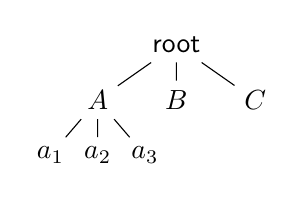
\begin{tikzpicture}[level distance=7mm]
          \tikzstyle{level 1}=[sibling distance=10mm]
          \tikzstyle{level 2}=[sibling distance=6mm]
          \node {$\mathsf{root}$}
              child {node {$A$} child {node {$a_1$}} child {node {$a_2$}} child {node {$a_3$}}}
              child {node {$B$}}
              child {node {$C$}};
      \end{tikzpicture}
  };
  \node [rectangle,draw] (change1) at (5,3) {
      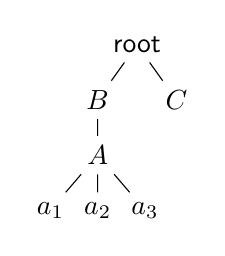
\begin{tikzpicture}[level distance=7mm]
          \tikzstyle{level 1}=[sibling distance=10mm]
          \tikzstyle{level 3}=[sibling distance=6mm]
          \node {$\mathsf{root}$}
              child {node {$B$} child {node {$A$} child {node {$a_1$}} child {node {$a_2$}} child {node {$a_3$}}}}
              child {node {$C$}};
      \end{tikzpicture}
  };
  \node [rectangle,draw] (change2) at (5,0) {
      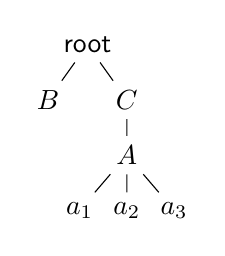
\begin{tikzpicture}[level distance=7mm]
          \tikzstyle{level 1}=[sibling distance=10mm]
          \tikzstyle{level 3}=[sibling distance=6mm]
          \node {$\mathsf{root}$}
              child {node {$B$}}
              child {node {$C$} child {node {$A$} child {node {$a_1$}} child {node {$a_2$}} child {node {$a_3$}}}};
      \end{tikzpicture}
  };
  \node [rectangle,draw,inner sep=3mm] (merge1) at (8.2,3) {?};
  \node [rectangle,draw,inner sep=3mm] (merge2) at (8.2,0) {?};
  \draw [time] (start1.east) -- node [above,text width=2.5cm,text centered,inner ysep=5pt] {Move $A$ to be a child of $B$} (change1.west);
  \draw [time] (change1.east) -- (merge1.west);
  \draw [time] (start2.east) -- node [above,text width=2.5cm,text centered,inner ysep=5pt] {Move $A$ to be a child of $C$} (change2.west);
  \draw [time] (change2.east) -- (merge2.west);
  \draw [network] (6.5,0) to [out=90,in=270] (7.2,3);
  \draw [network] (6.5,3) to [out=270,in=90] (7.2,0);
  \node [rotate=90,blue,font=\scriptsize] at (7.5,1.5) {network communication};
  \path [draw,dotted] (-3.1,1.5) -- (8.7,1.5);
  %%%
  \node [fill=red!15] at (9.63,4.10) {(\emph{a})};
  \node [fill=red!15] at (13.98,4.10) {(\emph{b})};
  \node [fill=red!15] at (9.64,1.10) {(\emph{c})};
  \node [fill=red!15] at (13.95,1.10) {(\emph{d})};
  \node [rectangle,draw] at (10.7,3) {
      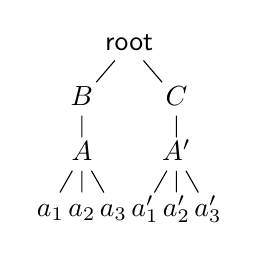
\begin{tikzpicture}[level distance=7mm]
          \tikzstyle{every node}=[text height=5pt,text depth=0pt]
          \tikzstyle{level 1}=[sibling distance=12mm]
          \tikzstyle{level 3}=[sibling distance=4mm]
          \node {$\mathsf{root}$}
              child {node {$B$} child {node {$A$} child {node {$a_1$}} child {node {$a_2$}} child {node {$a_3$}}}}
              child {node {$C$} child {node {$A'$} child {node {$a_1'$}} child {node {$a_2'$}} child {node {$a_3'$}}}};
      \end{tikzpicture}
  };
  \node [rectangle,draw] at (13.3,3) {
      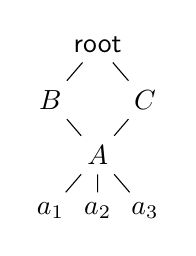
\begin{tikzpicture}[level distance=7mm]
          \tikzstyle{level 1}=[sibling distance=12mm]
          \node at (0,1.4) {$\mathsf{root}$} child {node (b) {$B$}} child {node (c) {$C$}};
          \tikzstyle{level 1}=[sibling distance=6mm]
          \node (a) at (0,0) {$A$} child {node {$a_1$}} child {node {$a_2$}} child {node {$a_3$}};
          \draw (b) -- (a);
          \draw (c) -- (a);
      \end{tikzpicture}
  };
  \node [rectangle,draw] at (10.5,0) {
      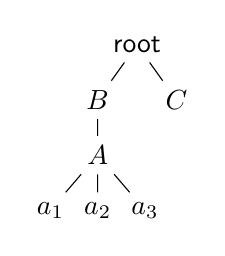
\begin{tikzpicture}[level distance=7mm]
          \tikzstyle{level 1}=[sibling distance=10mm]
          \tikzstyle{level 3}=[sibling distance=6mm]
          \node {$\mathsf{root}$}
              child {node {$B$} child {node {$A$} child {node {$a_1$}} child {node {$a_2$}} child {node {$a_3$}}}}
              child {node {$C$}};
      \end{tikzpicture}
  };
  \node [rectangle,draw] at (13.1,0) {
      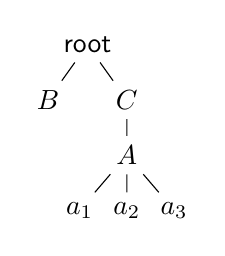
\begin{tikzpicture}[level distance=7mm]
          \tikzstyle{level 1}=[sibling distance=10mm]
          \tikzstyle{level 3}=[sibling distance=6mm]
          \node {$\mathsf{root}$}
              child {node {$B$}}
              child {node {$C$} child {node {$A$} child {node {$a_1$}} child {node {$a_2$}} child {node {$a_3$}}}};
      \end{tikzpicture}
  };
\end{tikzpicture}
\caption{Replica 1 moves $A$ to be a child of $B$, while concurrently replica 2 moves the same node $A$ to be a child of $C$. Boxes (\emph{a}) to (\emph{d}) show possible outcomes after the replicas have communicated and merged their states.}
\label{fig:move-same-item}
\end{figure*}

\begin{figure*}
\centering
\begin{tikzpicture}
  \tikzstyle{time}=[thick,->,gray]
  \tikzstyle{network}=[thick,dashed,blue,-{Stealth[length=3mm]}]
  \node [anchor=east] at (-1.2,3) {Replica 1:};
  \node [anchor=east] at (-1.2,0) {Replica 2:};
  \node [rectangle,draw] (start1) at (0,3) {
      \begin{tikzpicture}[level distance=7mm]
      \node {$\mathsf{root}$} child {node {$A$} child {node {$C$}}} child {node {$B$}};
      \end{tikzpicture}
  };
  \node [rectangle,draw] (start2) at (0,0) {
      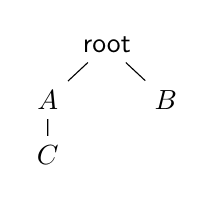
\begin{tikzpicture}[level distance=7mm]
      \node {$\mathsf{root}$} child {node {$A$} child {node {$C$}}} child {node {$B$}};
      \end{tikzpicture}
  };
  \node [rectangle,draw] (change1) at (4.5,3) {
      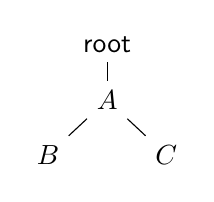
\begin{tikzpicture}[level distance=7mm]
      \node {$\mathsf{root}$} child {node {$A$} child {node {$B$}} child {node {$C$}}};
      \end{tikzpicture}
  };
  \node [rectangle,draw] (change2) at (4.5,0) {
      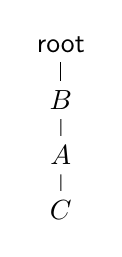
\begin{tikzpicture}[level distance=7mm]
      \node {$\mathsf{root}$} child {node {$B$} child {node {$A$} child {node {$C$}}}};
      \end{tikzpicture}
  };
  \node [rectangle,draw,inner sep=3mm] (merge1) at (8,3) {?};
  \node [rectangle,draw,inner sep=3mm] (merge2) at (8,0) {?};
  \draw [time] (start1.east) -- node [above,text width=2.5cm,text centered,inner ysep=5pt] {Move $B$ to be a child of $A$} (change1.west);
  \draw [time] (change1.east) -- (merge1.west);
  \draw [time] (start2.east) -- node [above,text width=2.5cm,text centered,inner ysep=5pt] {Move $A$ to be a child of $B$} (change2.west);
  \draw [time] (change2.east) -- (merge2.west);
  \draw [network] (6.0,0) to [out=90,in=270] (6.7,3);
  \draw [network] (6.0,3) to [out=270,in=90] (6.7,0);
  \node [rotate=90,blue,font=\scriptsize] at (7.0,1.5) {network communication};
  \path [draw,dotted] (-2.5,1.6) -- (8.5,1.6);
  %%%%%
  \node [rectangle,draw] at (10.75,3) {
      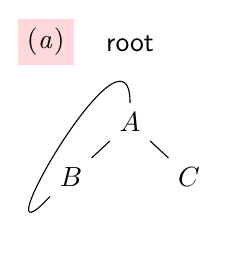
\begin{tikzpicture}[level distance=7mm]
      \useasboundingbox (-1.3,-1.3) rectangle (1,1.2);
      \node [fill=red!15] at (-1.07,1.02) {(\emph{a})};
      \node at (0,1) {$\mathsf{root}$};
      \node (a1) {$A$} child {node (b1) {$B$}} child {node {$C$}};
      \draw (b1.south west) .. controls (-2,-2) and (0,1.5) .. (a1.north);
      \end{tikzpicture}
  };
  \node [rectangle,draw] at (13.6,3) {
      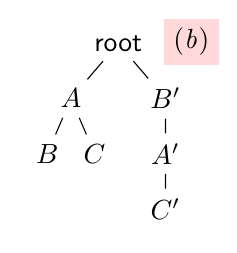
\begin{tikzpicture}[level distance=7mm]
      \useasboundingbox (-1.15,-2.3) rectangle (1.15,0.2);
      \node [fill=red!15] at (0.93,0.02) {(\emph{b})};
      \tikzstyle{level 1}=[sibling distance=12mm]
      \tikzstyle{level 2}=[sibling distance=6mm]
      \node {$\mathsf{root}$}
          child {node {$A$} child {node {$B$}} child {node {$C$}}}
          child {node {$B'$} child {node {$A'$} child {node {$C'$}}}};
      \end{tikzpicture}
  };
  \node [rectangle,draw] (start) at (10.75,0) {
      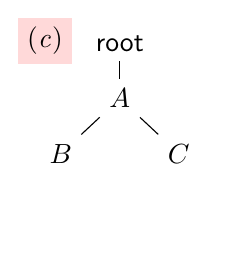
\begin{tikzpicture}[level distance=7mm]
      \useasboundingbox (-1.17,-2.3) rectangle (1.15,0.2);
      \node [fill=red!15] at (-0.95,0.03) {(\emph{c})};
      \node {$\mathsf{root}$} child {node {$A$} child {node {$B$}} child {node {$C$}}};
      \end{tikzpicture}
  };
  \node [rectangle,draw] (right) at (13.6,0) {
      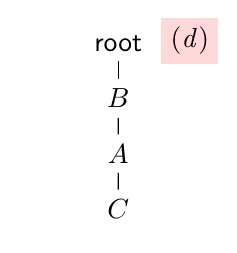
\begin{tikzpicture}[level distance=7mm]
      \useasboundingbox (-1.15,-2.3) rectangle (1.15,0.2);
      \node [fill=red!15] at (0.91,0.03) {(\emph{d})};
      \node {$\mathsf{root}$} child {node {$B$} child {node {$A$} child {node {$C$}}}};
      \end{tikzpicture}
  };
\end{tikzpicture}
\caption{Initially, nodes $A$ and $B$ are siblings. Replica 1 moves $B$ to be a child of $A$, while concurrently replica 2 moves $A$ to be a child of $B$. Boxes (\emph{a}) to (\emph{d}) show possible outcomes after the replicas have communicated and merged their states.}\label{fig:move-cycle}
\end{figure*}

\begin{figure*}
  \centering
  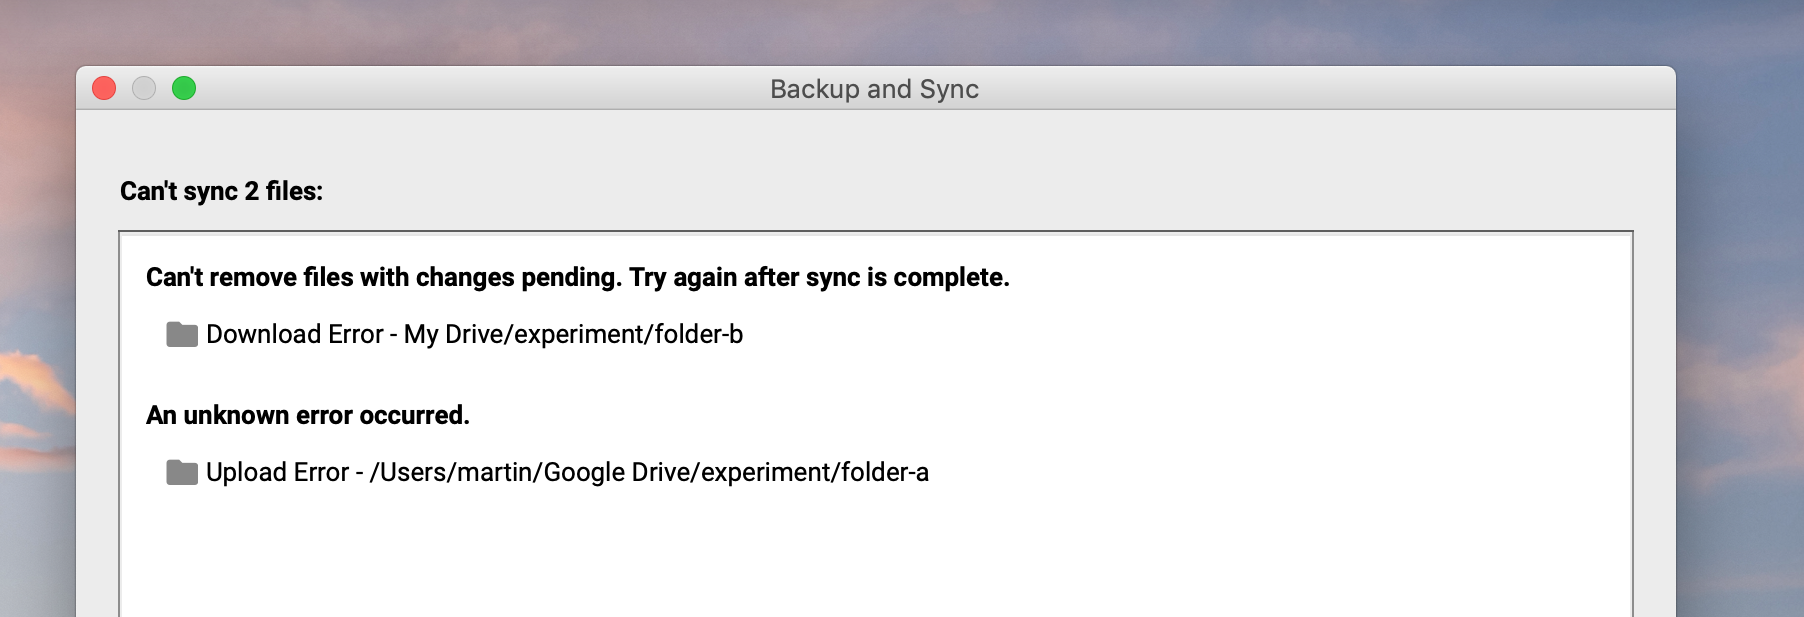
\includegraphics[width=\textwidth,keepaspectratio=true]{gdrive-error.png}
  \caption{Error message produced by Google Drive Backup and Sync on Mac OS as a result of performing the operations shown in Figure~\ref{fig:move-cycle}, indicating a bug in the underlying sync implementation.}
  \label{fig:gdrive-error}
\end{figure*}

\section{Why a move operation is hard}\label{sec:move-is-hard}

Applications that rely on a tree data model often need to move a node from one location to another location within the tree, such that all of its children move along with it:
\begin{itemize}
    \item In a filesystem, any file or directory can be moved to a different parent directory.
        Moreover, renaming a file or directory is equivalent to moving it to a new name without changing its parent directory.
    \item In a rich text editor, a paragraph can be turned into a bullet point.
        In the XML tree this corresponds to creating new list and bullet point nodes, and then moving the paragraph node inside the bullet point.
    \item In presentation software, grouping two graphical objects corresponds to creating a new group node, and then moving the two objects into the new group node.
\end{itemize}
As these operations are so common, it is not obvious why a move operation should be difficult in a replicated setting.
In this section we demonstrate some problems that arise with replicated trees, before proceeding to our solution in \S\ref{sec:algorithm}.

\subsection{Concurrent moves of the same node}\label{sec:move-same-item}

The first difficulty arises when the same node is concurrently moved into different locations on different replicas.
This scenario is illustrated in Figure~\ref{fig:move-same-item}, where replica 1 moves node $A$ to be a child of $B$, while concurrently replica 2 moves $A$ to be a child of $C$.
After the replicas communicate, what should the merged state of the tree be?

If a move operation is implemented by deleting the moved subtree from its old location, and then re-creating it at the new location, the merged state will be as shown in Figure~\ref{fig:move-same-item}a: the concurrent moves will duplicate the moved subtree, since each move independently recreates the subtree in each destination location.
We believe that this duplication is undesirable, since subsequent edits to nodes in the duplicated subtree will apply to only one of the copies.
Two users who believe they are collaborating on the same file may in fact be editing two different copies, which will then become inconsistent with each other.
In the rich text editor and presentation software examples, such duplication is also undesirable.

Another possible resolution is for the destination locations of both moves to refer to the same node, as shown in Figure~\ref{fig:move-same-item}b.
However, the result is a DAG, not a tree.
POSIX filesystems do not allow this outcome, since they do not allow hardlinks to directories.

In our opinion, the only reasonable outcomes are those shown in Figure~\ref{fig:move-same-item}c and~\ref{fig:move-same-item}d: the moved subtree appears either in replica 1's destination location or in replica 2's destination location, but not in both.
Which one of these two is picked is arbitrary, due to the symmetry between the two replicas.
The ``winning'' location could be picked based on a timestamp in the operations, similarly to the ``last writer wins'' conflict resolution method of Thomas's write rule~\cite{Johnson:1975we}.
(The \emph{timestamp} in this context need not come from a physical clock; it could also be logical, such as a Lamport timestamp~\cite{Lamport:1978jq}.)

We tested this scenario with file sync products Dropbox and Google Drive by concurrently moving the same directory to two different destination directories.\footnote{Experiment setup: we installed the official Mac OS clients for Dropbox and Google Drive on two computers, logged into the same Dropbox/Google accounts, and configured them to sync a directory on the local filesystem.
To test concurrent operations, we disconnected both computers from the Internet, performed a move operation on the local filesystem of each computer, then reconnected and waited for them to sync.}
Dropbox exhibited the undesirable duplication behaviour of Figure~\ref{fig:move-same-item}a, while the outcome on Google Drive was as in Figure~\ref{fig:move-same-item}c/d.

\subsection{Moving a node to be a descendant of itself}\label{sec:move-cycle}

On a filesystem, the destination directory of a move operation must not be a subdirectory of the directory being moved.
For example, if \texttt{b} is a subdirectory of \texttt{a}, then the Unix shell command \texttt{mv a a/b/} will fail with an error.
This restriction is required because allowing this operation would introduce a cycle into the directory graph, and so the filesystem would no longer be a tree.
The same restriction is required in any other tree structure that supports a move operation.

In an unreplicated tree it is easy to prevent cycles being introduced: if the node being moved is an ancestor of the destination node, the operation is rejected.
However, in a replicated setting, different replicas may perform operations that are individually safe, but whose combination leads to a cycle.
One such example is illustrated in Figure~\ref{fig:move-cycle}.
Here, replica 1 moves $B$ to be a child of $A$, while concurrently replica 2 moves $A$ to be a child of $B$.
As each replica propagates its operation to the other replica, a careless implementation might end up in the state shown in Figure~\ref{fig:move-cycle}a, in which $A$ and $B$ have formed a cycle, detached from the tree.

Another possible resolution is shown in Figure~\ref{fig:move-cycle}b: the nodes involved in the concurrent moves (and their children) could be duplicated, so that both ``$A$ as a child of $B$'' and ``$B$ as a child of $A$'' can exist in the tree.
However, such duplication is undesirable for the same reasons as in \S\ref{sec:move-same-item}.

In our opinion, the best way of handling the conflicting operations of Figure~\ref{fig:move-cycle} is to choose either Figure~\ref{fig:move-cycle}c or~\ref{fig:move-cycle}d: that is, either the result of applying replica 1's operation and ignoring replica 2's operation, or vice versa.
Like in \S\ref{sec:move-same-item}, the winning operation can be picked based on a timestamp.

As before, we tested this scenario with Google Drive and Dropbox.
In Google Drive, one replica was able to successfully sync with the server, while the other replica displayed the ``unknown error'' message shown in Figure~\ref{fig:gdrive-error}.
The replica in an error state refused to sync the conflicting directory, and its filesystem state remained permanently inconsistent with the other replica.
This error state persisted until the directories on the erroring replica were manually moved to match the state of the other replica.
On the other hand, Dropbox exhibited the duplication behaviour shown in Figure~\ref{fig:move-cycle}b.

\subsection{A highly-available move operation: impossible?}\label{sec:impossibility}

Najafzadeh et al.~\cite{Najafzadeh:2017vk,Najafzadeh:2018bw} previously implemented a replicated filesystem with a move operation, and analysed the case of concurrent move operations introducing a cycle.
Using the CISE proof tool~\cite{DBLP:conf/popl/GotsmanYFNS16,Najafzadeh:2016fi} the authors confirm that it is not sufficient for the replica that generates a move operation to check whether the operation introduces a cycle: like in Figure~\ref{fig:move-cycle}, two concurrent operations may be safe individually, but introduce a cycle when combined.

Najafzadeh et al. propose two solutions to this problem: either to duplicate tree nodes, as in Figure~\ref{fig:move-cycle}b, or to execute a synchronous locking protocol that prevents two move operations from concurrently modifying the same part of the tree.
The downside of a locking protocol is that the move operation is no longer highly available in the presence of network partitions, since it must wait for synchronous communication with other replicas or a lock server.

While these solutions are valid, the authors go on to claim that ``no file system can support an unsynchronised move without anomalies, such as loss or duplication''~\cite{Najafzadeh:2018bw}.
We refute that claim in this paper: our algorithm does not perform any locking, coordination or synchronisation among replicas, but it nevertheless ensures that the tree invariants are always satisfied (in particular, it never introduces cycles), and it never duplicates or loses any tree nodes.
To our knowledge, our algorithm is the first to provide all of these properties simultaneously.
We give a precise specification of our algorithm's consistency properties in \S\ref{sec:proof}.


\begin{figure*}
\raggedright
\begin{isabellebody}
\internallinenumbers\setstretch{1.2}
\isacommand{datatype}\isamarkupfalse%
\ {\isacharparenleft}{\isacharprime}t{\isacharcomma}\ {\isacharprime}n{\isacharcomma}\ {\isacharprime}m{\isacharparenright}\ operation\isanewline
\ \ {\isacharequal}\ Move\ {\isacharparenleft}move{\isacharunderscore}time{\isacharcolon}\ {\isacharprime}t{\isacharparenright}\isanewline
\ \ \ \ \ \ \ \ \ {\isacharparenleft}move{\isacharunderscore}parent{\isacharcolon}\ {\isacharprime}n{\isacharparenright}\isanewline
\ \ \ \ \ \ \ \ \ {\isacharparenleft}move{\isacharunderscore}meta{\isacharcolon}\ {\isacharprime}m{\isacharparenright}\isanewline
\ \ \ \ \ \ \ \ \ {\isacharparenleft}move{\isacharunderscore}child{\isacharcolon}\ {\isacharprime}n{\isacharparenright}\isanewline
\isanewline
\isacommand{datatype}\isamarkupfalse%
\ {\isacharparenleft}{\isacharprime}t{\isacharcomma}\ {\isacharprime}n{\isacharcomma}\ {\isacharprime}m{\isacharparenright}\ log{\isacharunderscore}op\isanewline
\ \ {\isacharequal}\ LogMove\ {\isacharparenleft}log{\isacharunderscore}time{\isacharcolon}\ {\isacharprime}t{\isacharparenright}\isanewline
\ \ \ \ \ \ \ \ \ \ \ \ {\isacharparenleft}old{\isacharunderscore}parent{\isacharcolon}\ {\isacartoucheopen}{\isacharparenleft}{\isacharprime}n\ {\isasymtimes}\ {\isacharprime}m{\isacharparenright}\ option{\isacartoucheclose}{\isacharparenright}\isanewline
\ \ \ \ \ \ \ \ \ \ \ \ {\isacharparenleft}new{\isacharunderscore}parent{\isacharcolon}\ {\isacharprime}n{\isacharparenright}\isanewline
\ \ \ \ \ \ \ \ \ \ \ \ {\isacharparenleft}log{\isacharunderscore}meta{\isacharcolon}\ {\isacharprime}m{\isacharparenright}\isanewline
\ \ \ \ \ \ \ \ \ \ \ \ {\isacharparenleft}log{\isacharunderscore}child{\isacharcolon}\ {\isacharprime}n{\isacharparenright}\isanewline
\isanewline
\isacommand{type{\isacharunderscore}synonym}\isamarkupfalse%
\ {\isacharparenleft}{\isacharprime}t{\isacharcomma}\ {\isacharprime}n{\isacharcomma}\ {\isacharprime}m{\isacharparenright}\ state\ {\isacharequal}\ {\isacartoucheopen}{\isacharparenleft}{\isacharprime}t{\isacharcomma}\ {\isacharprime}n{\isacharcomma}\ {\isacharprime}m{\isacharparenright}\ log{\isacharunderscore}op\ list\ {\isasymtimes}\ {\isacharparenleft}{\isacharprime}n\ {\isasymtimes}\ {\isacharprime}m\ {\isasymtimes}\ {\isacharprime}n{\isacharparenright}\ set{\isacartoucheclose}\isanewline
\isanewline
\isacommand{definition}\isamarkupfalse%
\ get{\isacharunderscore}parent\ {\isacharcolon}{\isacharcolon}\ {\isacartoucheopen}{\isacharparenleft}{\isacharprime}n\ {\isasymtimes}\ {\isacharprime}m\ {\isasymtimes}\ {\isacharprime}n{\isacharparenright}\ set\ {\isasymRightarrow}\ {\isacharprime}n\ {\isasymRightarrow}\ {\isacharparenleft}{\isacharprime}n\ {\isasymtimes}\ {\isacharprime}m{\isacharparenright}\ option{\isacartoucheclose}\ \isakeyword{where}\isanewline
\ \ {\isacartoucheopen}get{\isacharunderscore}parent\ tree\ child\ {\isasymequiv}\isanewline
\ \ \ \ \ if\ {\isasymexists}{\isacharbang}parent{\isachardot}\ {\isasymexists}{\isacharbang}meta{\isachardot}\ {\isacharparenleft}parent{\isacharcomma}\ meta{\isacharcomma}\ child{\isacharparenright}\ {\isasymin}\ tree\ then\isanewline
\ \ \ \ \ \ \ Some\ {\isacharparenleft}THE\ {\isacharparenleft}parent{\isacharcomma}\ meta{\isacharparenright}{\isachardot}\ {\isacharparenleft}parent{\isacharcomma}\ meta{\isacharcomma}\ child{\isacharparenright}\ {\isasymin}\ tree{\isacharparenright}\isanewline
\ \ \ \ \ else\ None{\isacartoucheclose}\isanewline
\isanewline
\isacommand{inductive}\isamarkupfalse%
\ ancestor\ {\isacharcolon}{\isacharcolon}\ {\isacartoucheopen}{\isacharparenleft}{\isacharprime}n\ {\isasymtimes}\ {\isacharprime}m\ {\isasymtimes}\ {\isacharprime}n{\isacharparenright}\ set\ {\isasymRightarrow}\ {\isacharprime}n\ {\isasymRightarrow}\ {\isacharprime}n\ {\isasymRightarrow}\ bool{\isacartoucheclose}\ \isakeyword{where}\isanewline
\ \ {\isacartoucheopen}{\isasymlbrakk}{\isacharparenleft}parent{\isacharcomma}\ meta{\isacharcomma}\ child{\isacharparenright}\ {\isasymin}\ tree{\isasymrbrakk}\ {\isasymLongrightarrow}\ ancestor\ tree\ parent\ child{\isacartoucheclose}\ {\isacharbar}\isanewline
\ \ {\isacartoucheopen}{\isasymlbrakk}{\isacharparenleft}parent{\isacharcomma}\ meta{\isacharcomma}\ child{\isacharparenright}\ {\isasymin}\ tree{\isacharsemicolon}\ ancestor\ tree\ anc\ parent{\isasymrbrakk}\ {\isasymLongrightarrow}\ ancestor\ tree\ anc\ child{\isacartoucheclose}\isanewline
\isanewline
\isacommand{fun}\isamarkupfalse%
\ do{\isacharunderscore}op\ {\isacharcolon}{\isacharcolon}\ {\isacartoucheopen}{\isacharparenleft}{\isacharprime}t{\isacharcomma}\ {\isacharprime}n{\isacharcomma}\ {\isacharprime}m{\isacharparenright}\ operation\ {\isasymtimes}\ {\isacharparenleft}{\isacharprime}n\ {\isasymtimes}\ {\isacharprime}m\ {\isasymtimes}\ {\isacharprime}n{\isacharparenright}\ set\ {\isasymRightarrow}\isanewline
\ \ \ \ \ \ \ \ \ \ \ \ \ \ {\isacharparenleft}{\isacharprime}t{\isacharcomma}\ {\isacharprime}n{\isacharcomma}\ {\isacharprime}m{\isacharparenright}\ log{\isacharunderscore}op\ {\isasymtimes}\ {\isacharparenleft}{\isacharprime}n\ {\isasymtimes}\ {\isacharprime}m\ {\isasymtimes}\ {\isacharprime}n{\isacharparenright}\ set{\isacartoucheclose}\ \isakeyword{where}\isanewline
\ \ {\isacartoucheopen}do{\isacharunderscore}op\ {\isacharparenleft}Move\ t\ newp\ m\ c{\isacharcomma}\ tree{\isacharparenright}\ {\isacharequal}\isanewline
\ \ \ \ \ {\isacharparenleft}LogMove\ t\ {\isacharparenleft}get{\isacharunderscore}parent\ tree\ c{\isacharparenright}\ newp\ m\ c{\isacharcomma}\isanewline
\ \ \ \ \ \ if\ ancestor\ tree\ c\ newp\ {\isasymor}\ c\ {\isacharequal}\ newp\ then\ tree\isanewline
\ \ \ \ \ \ else\ {\isacharbraceleft}{\isacharparenleft}p{\isacharprime}{\isacharcomma}\ m{\isacharprime}{\isacharcomma}\ c{\isacharprime}{\isacharparenright}\ {\isasymin}\ tree{\isachardot}\ c{\isacharprime}\ {\isasymnoteq}\ c{\isacharbraceright}\ {\isasymunion}\ {\isacharbraceleft}{\isacharparenleft}newp{\isacharcomma}\ m{\isacharcomma}\ c{\isacharparenright}{\isacharbraceright}{\isacharparenright}{\isacartoucheclose}\isanewline
\isanewline
\isacommand{fun}\isamarkupfalse%
\ undo{\isacharunderscore}op\ {\isacharcolon}{\isacharcolon}\ {\isacartoucheopen}{\isacharparenleft}{\isacharprime}t{\isacharcomma}\ {\isacharprime}n{\isacharcomma}\ {\isacharprime}m{\isacharparenright}\ log{\isacharunderscore}op\ {\isasymtimes}\ {\isacharparenleft}{\isacharprime}n\ {\isasymtimes}\ {\isacharprime}m\ {\isasymtimes}\ {\isacharprime}n{\isacharparenright}\ set\ {\isasymRightarrow}\ {\isacharparenleft}{\isacharprime}n\ {\isasymtimes}\ {\isacharprime}m\ {\isasymtimes}\ {\isacharprime}n{\isacharparenright}\ set{\isacartoucheclose}\ \isakeyword{where}\isanewline
\ \ {\isacartoucheopen}undo{\isacharunderscore}op\ {\isacharparenleft}LogMove\ t\ None\ newp\ m\ c{\isacharcomma}\ tree{\isacharparenright}\ {\isacharequal}\ {\isacharbraceleft}{\isacharparenleft}p{\isacharprime}{\isacharcomma}\ m{\isacharprime}{\isacharcomma}\ c{\isacharprime}{\isacharparenright}\ {\isasymin}\ tree{\isachardot}\ c{\isacharprime}\ {\isasymnoteq}\ c{\isacharbraceright}{\isacartoucheclose}\ {\isacharbar}\isanewline
\ \ {\isacartoucheopen}undo{\isacharunderscore}op\ {\isacharparenleft}LogMove\ t\ {\isacharparenleft}Some\ {\isacharparenleft}oldp{\isacharcomma}\ oldm{\isacharparenright}{\isacharparenright}\ newp\ m\ c{\isacharcomma}\ tree{\isacharparenright}\ {\isacharequal}\isanewline
\ \ \ \ \ {\isacharbraceleft}{\isacharparenleft}p{\isacharprime}{\isacharcomma}\ m{\isacharprime}{\isacharcomma}\ c{\isacharprime}{\isacharparenright}\ {\isasymin}\ tree{\isachardot}\ c{\isacharprime}\ {\isasymnoteq}\ c{\isacharbraceright}\ {\isasymunion}\ {\isacharbraceleft}{\isacharparenleft}oldp{\isacharcomma}\ oldm{\isacharcomma}\ c{\isacharparenright}{\isacharbraceright}{\isacartoucheclose}\isanewline
\isanewline
\isacommand{fun}\isamarkupfalse%
\ redo{\isacharunderscore}op\ {\isacharcolon}{\isacharcolon}\ {\isacartoucheopen}{\isacharparenleft}{\isacharprime}t{\isacharcomma}\ {\isacharprime}n{\isacharcomma}\ {\isacharprime}m{\isacharparenright}\ log{\isacharunderscore}op\ {\isasymRightarrow}\ {\isacharparenleft}{\isacharprime}t{\isacharcomma}\ {\isacharprime}n{\isacharcomma}\ {\isacharprime}m{\isacharparenright}\ state\ {\isasymRightarrow}\ {\isacharparenleft}{\isacharprime}t{\isacharcomma}\ {\isacharprime}n{\isacharcomma}\ {\isacharprime}m{\isacharparenright}\ state{\isacartoucheclose}\ \isakeyword{where}\isanewline
\ \ {\isacartoucheopen}redo{\isacharunderscore}op\ {\isacharparenleft}LogMove\ t\ {\isacharunderscore}\ p\ m\ c{\isacharparenright}\ {\isacharparenleft}ops{\isacharcomma}\ tree{\isacharparenright}\ {\isacharequal}\isanewline
\ \ \ \ \ {\isacharparenleft}let\ {\isacharparenleft}op{\isadigit{2}}{\isacharcomma}\ tree{\isadigit{2}}{\isacharparenright}\ {\isacharequal}\ do{\isacharunderscore}op\ {\isacharparenleft}Move\ t\ p\ m\ c{\isacharcomma}\ tree{\isacharparenright}\isanewline
\ \ \ \ \ \ in\ {\isacharparenleft}op{\isadigit{2}}\ {\isacharhash}\ ops{\isacharcomma}\ tree{\isadigit{2}}{\isacharparenright}{\isacharparenright}{\isacartoucheclose}\isanewline
\isanewline
\isacommand{fun}\isamarkupfalse%
\ apply{\isacharunderscore}op\ {\isacharcolon}{\isacharcolon}\ {\isacartoucheopen}{\isacharparenleft}{\isacharprime}t{\isacharcolon}{\isacharcolon}{\isacharbraceleft}linorder{\isacharbraceright}{\isacharcomma}\ {\isacharprime}n{\isacharcomma}\ {\isacharprime}m{\isacharparenright}\ operation\ {\isasymRightarrow}\isanewline
\ \ \ \ \ \ \ \ \ \ \ \ \ \ \ \ \ \ {\isacharparenleft}{\isacharprime}t{\isacharcomma}\ {\isacharprime}n{\isacharcomma}\ {\isacharprime}m{\isacharparenright}\ state\ {\isasymRightarrow}\ {\isacharparenleft}{\isacharprime}t{\isacharcomma}\ {\isacharprime}n{\isacharcomma}\ {\isacharprime}m{\isacharparenright}\ state{\isacartoucheclose}\ \isakeyword{where}\isanewline
\ \ {\isacartoucheopen}apply{\isacharunderscore}op\ op{\isadigit{1}}\ {\isacharparenleft}{\isacharbrackleft}{\isacharbrackright}{\isacharcomma}\ tree{\isadigit{1}}{\isacharparenright}\ {\isacharequal}\isanewline
\ \ \ \ \ {\isacharparenleft}let\ {\isacharparenleft}op{\isadigit{2}}{\isacharcomma}\ tree{\isadigit{2}}{\isacharparenright}\ {\isacharequal}\ do{\isacharunderscore}op\ {\isacharparenleft}op{\isadigit{1}}{\isacharcomma}\ tree{\isadigit{1}}{\isacharparenright}\isanewline
\ \ \ \ \ \ in\ {\isacharparenleft}{\isacharbrackleft}op{\isadigit{2}}{\isacharbrackright}{\isacharcomma}\ tree{\isadigit{2}}{\isacharparenright}{\isacharparenright}{\isacartoucheclose}\ {\isacharbar}\isanewline
\ \ {\isacartoucheopen}apply{\isacharunderscore}op\ op{\isadigit{1}}\ {\isacharparenleft}logop\ {\isacharhash}\ ops{\isacharcomma}\ tree{\isadigit{1}}{\isacharparenright}\ {\isacharequal}\isanewline
\ \ \ \ \ {\isacharparenleft}if\ move{\isacharunderscore}time\ op{\isadigit{1}}\ {\isacharless}\ log{\isacharunderscore}time\ logop\isanewline
\ \ \ \ \ \ then\ redo{\isacharunderscore}op\ logop\ {\isacharparenleft}apply{\isacharunderscore}op\ op{\isadigit{1}}\ {\isacharparenleft}ops{\isacharcomma}\ undo{\isacharunderscore}op\ {\isacharparenleft}logop{\isacharcomma}\ tree{\isadigit{1}}{\isacharparenright}{\isacharparenright}{\isacharparenright}\isanewline
\ \ \ \ \ \ else\ let\ {\isacharparenleft}op{\isadigit{2}}{\isacharcomma}\ tree{\isadigit{2}}{\isacharparenright}\ {\isacharequal}\ do{\isacharunderscore}op\ {\isacharparenleft}op{\isadigit{1}}{\isacharcomma}\ tree{\isadigit{1}}{\isacharparenright}\ in\ {\isacharparenleft}op{\isadigit{2}}\ {\isacharhash}\ logop\ {\isacharhash}\ ops{\isacharcomma}\ tree{\isadigit{2}}{\isacharparenright}{\isacharparenright}{\isacartoucheclose}\isanewline
\isanewline
\isacommand{definition}\isamarkupfalse%
\ apply{\isacharunderscore}ops\ {\isacharcolon}{\isacharcolon}\ {\isacartoucheopen}{\isacharparenleft}{\isacharprime}t{\isacharcolon}{\isacharcolon}{\isacharbraceleft}linorder{\isacharbraceright}{\isacharcomma}\ {\isacharprime}n{\isacharcomma}\ {\isacharprime}m{\isacharparenright}\ operation\ list\ {\isasymRightarrow}\ {\isacharparenleft}{\isacharprime}t{\isacharcomma}\ {\isacharprime}n{\isacharcomma}\ {\isacharprime}m{\isacharparenright}\ state{\isacartoucheclose}\ \isakeyword{where}\isanewline
\ \ {\isacartoucheopen}apply{\isacharunderscore}ops\ ops\ {\isasymequiv}\ foldl\ {\isacharparenleft}{\isasymlambda}state\ oper{\isachardot}\ apply{\isacharunderscore}op\ oper\ state{\isacharparenright}\ {\isacharparenleft}{\isacharbrackleft}{\isacharbrackright}{\isacharcomma}\ {\isacharbraceleft}{\isacharbraceright}{\isacharparenright}\ ops{\isacartoucheclose}\isanewline
\isanewline
\isacommand{definition}\isamarkupfalse%
\ unique{\isacharunderscore}parent\ {\isacharcolon}{\isacharcolon}\ {\isacartoucheopen}{\isacharparenleft}{\isacharprime}n\ {\isasymtimes}\ {\isacharprime}m\ {\isasymtimes}\ {\isacharprime}n{\isacharparenright}\ set\ {\isasymRightarrow}\ bool{\isacartoucheclose}\ \isakeyword{where}\isanewline
\ \ {\isacartoucheopen}unique{\isacharunderscore}parent\ tree\ {\isasymequiv}\ {\isacharparenleft}{\isasymforall}p{\isadigit{1}}\ p{\isadigit{2}}\ m{\isadigit{1}}\ m{\isadigit{2}}\ c{\isachardot}\ {\isacharparenleft}p{\isadigit{1}}{\isacharcomma}\ m{\isadigit{1}}{\isacharcomma}\ c{\isacharparenright}\ {\isasymin}\ tree\ {\isasymand}\ {\isacharparenleft}p{\isadigit{2}}{\isacharcomma}\ m{\isadigit{2}}{\isacharcomma}\ c{\isacharparenright}\ {\isasymin}\ tree\ {\isasymlongrightarrow}\ p{\isadigit{1}}\ {\isacharequal}\ p{\isadigit{2}}\ {\isasymand}\ m{\isadigit{1}}\ {\isacharequal}\ m{\isadigit{2}}{\isacharparenright}{\isacartoucheclose}\isanewline%
\isanewline
\isacommand{definition}\isamarkupfalse%
\ acyclic\ {\isacharcolon}{\isacharcolon}\ {\isacartoucheopen}{\isacharparenleft}{\isacharprime}n\ {\isasymtimes}\ {\isacharprime}m\ {\isasymtimes}\ {\isacharprime}n{\isacharparenright}\ set\ {\isasymRightarrow}\ bool{\isacartoucheclose}\ \isakeyword{where}\isanewline
\ \ {\isacartoucheopen}acyclic\ tree\ {\isasymequiv}\ {\isacharparenleft}{\isasymnexists}n{\isachardot}\ ancestor\ tree\ n\ n{\isacharparenright}{\isacartoucheclose}
\end{isabellebody}
\caption{The move operation algorithm, implemented in the Isabelle/HOL language.}
\label{fig:code}
\end{figure*}

\section{The replicated move operation}\label{sec:algorithm}

We now introduce our algorithm for a replicated tree that supports a move operation.
We model each replica as a state machine that transitions from one state to the next by applying an operation.
The algorithm is executed independently on each replica with no shared memory between replicas.

When the user wants to make a change to the tree, they generate an operation and apply it to their local replica.
Every operation is also asynchronously sent over the network to all other replicas, and applied to every remote replica using the same algorithm as for local operations.
The network may deliver operations in any order; thus, the communication can be performed peer-to-peer, and it does not require any central server or consensus protocol.
We only assume that eventually every operation is applied on every replica, provided that network partitions are of a finite duration.

The key consistency property of our algorithm is \emph{convergence}: that is, whenever any two replicas have applied the same set of operations, then they must be in the same state---even if the operations were applied in a different order on different replicas.
We prove this in \S\ref{sec:proof} by showing that applying operations is commutative.

Figure~\ref{fig:code} gives the full source code for our algorithm in the Isabelle/HOL language~\cite{DBLP:conf/tphol/WenzelPN08}.
We choose this language because it combines the conciseness of pseudocode with the precision of mathematical notation.
It supports formal reasoning, allowing us to prove the correctness of the algorithm (\S\ref{sec:proof}), and it can be exported to Scala, Haskell, or OCaml.

In this section we walk through the code in Figure~\ref{fig:code} step by step, explaining the Isabelle/HOL syntax as we encounter it.
Additional background documentation is available~\cite{DBLP:books/sp/NipkowK14}.

\subsection{Operations and trees}\label{sec:ops-trees}

We define one kind of operation: \isa{Move t p m c} (line 1--5).
A move operation is a 4-tuple consisting of a timestamp \isa{t} of type \isa{'t}, a parent node ID \isa{p} of type \isa{'n}, a metadata field \isa{m} of type \isa{'m}, and a child node ID \isa{c} of type \isa{'n}.
Here, \isa{'t}, \isa{'n} and \isa{'m} are \emph{type variables} that can be replaced with arbitrary types; we only require that node identifiers \isa{'n} are globally unique (e.g.\ UUIDs~\cite{Leach:2005hm}); timestamps \isa{'t} need to be globally unique and totally ordered (e.g. Lamport timestamps~\cite{Lamport:1978jq}).

The meaning of an operation \isa{Move t p m c} is that at time \isa{t}, the node with ID \isa{c} is moved to be a child of the parent node with ID \isa{p}.
The operation does not specify the old location of \isa{c}; the algorithm simply removes \isa{c} from wherever it is currently located in the tree, and moves it to \isa{p}.
If \isa{c} does not currently exist in the tree, it is created as a child of \isa{p}.
For this reason we do not need a separate operation type to create tree nodes: simply performing a move with a fresh child node ID \isa{c} is sufficient to create \isa{c}.
To delete \isa{c}, we move \isa{c} to be a child of the ``trash'' (a designated node ID that does not exist in the tree), so \isa{c} is removed from the tree.

The metadata field \isa{m} in a move operation allows additional information to be associated with the parent-child relationship of \isa{p} and \isa{c}.
For example, in a filesystem, the parent and child would be the inodes of a directory and a file within it, respectively, and the metadata would contain the filename of the child.
Thus, a file with inode \isa{c} can be renamed by performing a \isa{Move t p m c}, where the new parent directory \isa{p} is the unchanged inode of the existing parent directory, but the metadata \isa{m} contains the new filename.

When users want to make changes to the tree on their local replica, they generate new \isa{Move t p m c} operations for these changes, and apply these operations to their local replica using the algorithm described in the rest of this section.

We can represent the tree as a set of \isa{(parent, meta, child)} triples, denoted in Isabelle/HOL as \isa{('n {\isasymtimes} 'm {\isasymtimes} 'n) set}.
When we have \isa{(p, m, c) {\isasymin} tree}, that means \isa{c} is a child of \isa{p} in the tree, with associated metadata \isa{m}.
Given a \isa{tree}, we can construct a new \isa{tree'} in which the child \isa{c} is moved to a new parent \isa{p}, with associated metadata \isa{m}, as follows:
\begin{isabelle}
tree' = \{(p', m', c') {\isasymin} tree. c' {\isasymnoteq} c\} {\isasymunion} \{(p, m, c)\}
\end{isabelle}
That is, we remove any existing parent-child relationship for \isa{c} from the set \isa{tree}, and then add \isa{\{(p, m, c)\}} to represent the new parent-child relationship.
This expression appears on lines 31 and 36 of Figure~\ref{fig:code}, as we shall explain shortly.

\subsection{Replica state and operation log}\label{sec:state-log}

In order to correctly apply move operations, a replica needs to maintain not only the current state of the tree, but also an \emph{operation log}.
The log is a list of \isa{LogMove} records in descending timestamp order.
\isa{LogMove t oldp p m c} (lines 7--12) is similar to \isa{Move t p m c}; the difference is that \isa{LogMove} has an additional field \isa{oldp} of type \isa{('n {\isasymtimes} 'm) option}.
This \isa{option} type means the field can either take the value \isa{None} (similar to null), or a pair of a node ID and a metadata field.

When a replica applies a \isa{Move} operation to its tree, it also records a corresponding \isa{LogMove} operation in its log.
The \isa{t}, \isa{p}, \isa{m} and \isa{c} fields are taken directly from the \isa{Move} record, while the \isa{oldp} field is filled in based on the state of the tree before the move.
If \isa{c} did not exist in the tree, \isa{oldp} is set to \isa{None}.
Otherwise, \isa{oldp} records the previous parent and metadata of \isa{c}: if there exist \isa{p'} and \isa{m'} such that \isa{(p', m', c) {\isasymin} tree}, then \isa{oldp} is set to \isa{Some (p', m')}.
The \isa{get\_parent} function implements this (lines 16--20).

In the first line of \isa{get\_parent}, the expression between \isa{::} and \textbf{where} is the type signature of the function, in this case:
\begin{quote}
\isa{('n {\isasymtimes} 'm {\isasymtimes} 'n) set {\isasymRightarrow} 'n {\isasymRightarrow} ('n {\isasymtimes} 'm) option}
\end{quote}
This signature denotes a function that takes two arguments: a tree \isa{('n {\isasymtimes} 'm {\isasymtimes} 'n) set} and a node ID \isa{'n}.
It then returns a \isa{('n {\isasymtimes} 'm) option}.
The operator \isa{{\isasymexists}!x} means ``there exists a unique value \isa{x} such that\dots'', while \isa{THE x} means ``\emph{choose} the unique value \isa{x} such that\ldots''.

In line 14 we define the datatype for the state of a replica: a pair \isa{(log, tree)} where \isa{log} is a list of \isa{LogMove} records, and \isa{tree} is a set of \isa{(parent, meta, child)} triples as before.

\subsection{Preventing cycles}\label{sec:prevent-cycles}

Recall from \S\ref{sec:move-cycle} that in order to prevent a cycle being introduced, the node being moved must not be an ancestor of the destination node.
To implement this we first define the \isa{ancestor} relation in lines 22--24.
It is the transitive closure of a tree's parent-child relation: if \isa{(p, m, c) {\isasymin} tree} then \isa{p} is an ancestor of \isa{c} (line 23); moreover, if \isa{a} is an ancestor of \isa{p} and \isa{(p, m, c) {\isasymin} tree}, then \isa{a} is also an ancestor of \isa{c} (line 24).
The \textbf{inductive} keyword indicates that this recursive definition is iterated until the least fixed point is reached.

The \isa{do\_op} function (lines 26--31) now performs the actual work of applying a move operation.
This function takes as argument a pair consisting of a \isa{Move} operation and the current tree, and it returns a pair consisting of a \isa{LogMove} operation (which will be added to the log) and an updated tree.
In line 29, the \isa{LogMove} record is constructed as described in \S\ref{sec:state-log}, obtaining the prior parent and metadata of \isa{c} using the \isa{get\_parent} function.

Line 30 performs the check that ensures no cycles are introduced: if \isa{ancestor tree c newp}, i.e.\ if the node \isa{c} is being moved, and \isa{c} is an ancestor of the new parent \isa{newp}, then the tree is returned unmodified---in other words, the operation is ignored.
Similarly, the operation is also ignored if \isa{c = newp}.
Otherwise (line 31), the tree is updated by removing \isa{c} from its existing parent, if any, and adding the new parent-child relationship \isa{(newp, m, c)} to the tree.

\subsection{Applying operations in any order}\label{sec:applying}

The \isa{do\_op} function is sufficient for applying operations if all replicas apply operations in the same order.
However, in an optimistic replication setting, each replica may apply the operations in a different order, and we need to ensure that the replica state nevertheless converges towards a consistent state.
This goal is accomplished by the \isa{undo\_op}, \isa{redo\_op}, and \isa{apply\_op} functions (lines 33--51).

When a replica needs to apply an operation with timestamp \isa{t}, it first undoes the effect of any operations with a timestamp greater than \isa{t}, then performs the new operation, and finally re-applies the undone operations.
As a result, the state of the tree is as if the operations had all been applied in order of increasing timestamp, even though in fact they might have been applied in any order.

The \isa{apply\_op} function (lines 43--51) takes two arguments: a \isa{Move} operation to apply and the current replica state; and it returns the new replica state.
The \isa{'t::\{linorder\}} constraint in the type signature indicates that timestamps \isa{'t} are instances of \isa{linorder} type class, and they can therefore be compared with the \isa{<} operator defining a linear (or total) order.
This comparison occurs on line 49.

Recall that the replica state includes the operation log (line 14), and we use this log to perform the undo-do-redo cycle.
Lines 45--47 handle the case where the log is empty: in this case, we simply perform the operation using \isa{do\_op}, and return the new tree along with a log containing a single \isa{LogMove} record.
If the log is nonempty (line 48), we take \isa{logop} to be the first element of the log, and \isa{ops} to be the rest.
(The hash character in \isa{logop {\isacharhash} ops} is the \emph{list cons} operator that adds one element to the head of a list.)
If the timestamp of \isa{logop} is greater than the timestamp of the new operation (line 49) we first undo \isa{logop} with \isa{undo\_op}, then recursively apply the new operation to the remaining log, and finally reapply \isa{logop} with \isa{redo\_op} (line 50).
Otherwise we perform the operation using \isa{do\_op}, and add the corresponding \isa{LogMove} record as the head of the log (line 51).

This logic ensures that the log is maintained in descending timestamp order, with the greatest timestamp at the head.
\isa{undo\_op} (lines 33--36) inverts the effect of a previous move operation by restoring the prior parent and metadata that were recorded in the \isa{LogMove}'s additional field.
\isa{redo\_op} (lines 38--41) uses \isa{do\_op} to perform an operation again and recomputes the \isa{LogMove} record (which might have changed due to the effect of the new operation).

\subsection{Handling conflicts}\label{sec:conflicts}

Due to the undo-do-redo cycle, the state of the tree is as if all operations had been applied using \isa{do\_op} in increasing timestamp order, regardless of the order in which they were actually applied.
This provides a clear and consistent approach to the handling of conflicts:
\begin{itemize}
    \item If two operations concurrently move the same node, the operation with the lower timestamp moves the node first, and then the operation with the greater timestamp moves it again, so the final parent is determined by the latter.
        Since move operations do not specify the old location of a node, but only the new location, this sequential execution of concurrent operations is well-defined.
    \item If two operations would introduce a cycle when combined, as in \S\ref{sec:move-cycle}, then the operation with the greater timestamp is ignored.
        This is the case because \isa{do\_op} checks for cycles based on the tree created by all operations with a lower timestamp.
        The lower of two conflicting operations will take effect, since that operation by itself is safe.
        When the higher-timestamped operation is applied, \isa{do\_op} detects that it would introduce a cycle, and therefore ignores the operation.
\end{itemize}

Note that the safety of an operation (whether or not it would introduce a cycle) may change as subsequent operations with lower timestamps are applied.
For example, an operation may initially be regarded as safe, and then be reclassified as unsafe after applying a conflicting operation with a lower timestamp.
The opposite is also possible: an operation previously regarded as unsafe may become safe through the application of an operation that removes the risk of introducing a cycle.
For this reason, the operation log must include all operations, even those that were ignored.

One final type of conflict that we have not discussed so far is multiple child nodes with the same parent and the same metadata.
For example, in a filesystem, two users could concurrently create files with the same name in the same directory.
Our algorithm does not prevent such a conflict, but simply retains both child nodes.
In practice, the collision would be resolved by making the filenames distinct, e.g.\ by appending a replica identifier to the filenames.

\subsection{Algorithm extensions}\label{sec:extensions}

\noindent\textbf{Hardlinks and symlinks.}
Unix filesystems support hardlinks, which allow the same file inode to be referenced from multiple locations in a tree.
Our tree data structure can easily be extended to support this: rather than placing file data directly in the leaf nodes of the tree, the leaf node must reference the file inode.
Thus, references to the same file inode can appear in multiple leaf nodes of the tree.
Symlinks are also easy to support, since they are just leaf nodes containing a path (not a reference to an inode).

\smallbreak\noindent\textbf{Log truncation.}
The algorithm as specified in Figure~\ref{fig:code} retains operations in the log indefinitely, so the memory use grows without bound.
However, in practice it is easy to truncate the log, because \isa{apply\_op} only examines the log prefix of operations whose timestamp is greater than that of the operation being applied.
Thus, once it is known that all future operations will have a timestamp greater than $t$, then operations with timestamp $t$ or less can be discarded from the log.
In this case, we say that $t$ is \emph{causally stable}~\cite{Baquero:2014ed}.

A similar approach can be used to garbage-collect any tree nodes in the trash (\S\ref{sec:ops-trees}).
Initially, trashed nodes must be retained because a concurrent move operation may move them back out of the trash.
However, once the operation that moved a node to the trash is causally stable, we know that no future operations will refer to this node, and so the trashed node and its descendants can be discarded.

We can determine causal stability in a system where the set of replicas is known, where each replica generates operations with monotonically increasing timestamps, and where the communication link between any pair of replicas is FIFO (messages are received in the order in which they are sent, as implemented e.g.\ by TCP).
In this case, we can keep track of the most recent timestamp we have seen from each replica (including our own), and the minimum of these timestamps is the causally stable threshold.

\smallbreak\noindent\textbf{Ordering of sibling nodes.}
Another useful extension of the tree algorithm is to allow children of the same parent node to have an explicit ordering.
For example, in a graphics application, the order of nodes determines visibility (objects that are ``further back'' may be obscured by objects that are ``closer to the front'').
This can be implemented by maintaining an additional list CRDT for each branch node, e.g.\ using RGA~\cite{Roh:2011dw}, Treedoc~\cite{Preguica:2009fz}, Logoot~\cite{Weiss:2010hx}, or LSEQ~\cite{Nedelec:2013ky}.
These algorithms assign a unique ID to each element of the list, and this ID can be included in the metadata field of move operations in order to determine the order of sibling nodes.

This approach to determining ordering also easily supports reordering of child nodes within a parent, e.g.\ to implement the ``bring to front'' and ``send to back'' feature of applications like Microsoft PowerPoint.
To move a node to a different position in a list, we use the list CRDT to generate a new ID at the desired position in the sequence.
Then we perform a move operation in which the parent node is unchanged, but the metadata is changed to this new ID.

\smallbreak\noindent\textbf{File merging.}
In a distributed filesystem, replication and conflict resolution is required not only for the directory structure, but also for the contents of individual files.
This can be accomplished by using CRDTs for file contents as well.
We discuss distributed filesystems further in \S\ref{sec:filesystems}.

\section{Proof of correctness}\label{sec:proof}

We now discuss the correctness properties of the algorithm from \S\ref{sec:algorithm}.
All theorems stated here have been formally proved and mechanically checked using Isabelle.
For space reasons we give only a brief sketch of the proofs in this paper; the Isabelle files containing the full details are open source~\cite{SourceFiles}.

To reason about the state of a replica we first define the function \isa{apply\_ops} on lines 53--54 of Figure~\ref{fig:code}.
It takes a list of operations \isa{ops} and returns the state of a replica after it has applied all the operations in \isa{ops}.
The \isa{apply\_ops} function works by starting in the initial state \isa{([], \{\})} consisting of the empty operation log \isa{[]} and the tree represented by the empty set \isa{\{\}}, and then applying the operations one by one to the state using the \isa{apply\_op} function (introduced in \S\ref{sec:applying}).
The \isa{foldl} function from the Isabelle/HOL standard library performs the iteration over the list of operations.

\subsection{Tree invariants}\label{sec:tree-invariants}

A tree is an acyclic graph in which every node has exactly one parent, except for the root, which has no parent.
To prove that our algorithm maintains a tree structure, no matter which operations are applied, we prove that these invariants hold.
In fact, we slightly generalise this property and allow more than one root to exist, so the graph represents a forest, allowing an application to move nodes between different trees, if desired.
For example, the ``trash'' node used for deletion (\S\ref{sec:ops-trees}) can be separate from the main tree.

\subsubsection{Each node's parent is unique}\label{sec:unique-parent}

The first invariant we prove is that each tree node has either no parent (if it is the root of a tree) or exactly one parent (if it is a non-root node).
We state this theorem in Isabelle/HOL as follows, where \isa{apply\_ops\_unique\_parent} is the name we give to this theorem:
\begin{isabelle}
\isacommand{theorem}\isamarkupfalse%
\ apply{\isacharunderscore}ops{\isacharunderscore}unique{\isacharunderscore}parent{\isacharcolon}\isanewline
\ \ \isakeyword{assumes}\ {\isacartoucheopen}apply{\isacharunderscore}ops\ ops\ {\isacharequal}\ {\isacharparenleft}log{\isacharcomma}\ tree{\isacharparenright}{\isacartoucheclose}\isanewline
\ \ \isakeyword{shows}\ {\isacartoucheopen}unique{\isacharunderscore}parent\ tree{\isacartoucheclose}
\end{isabelle}
\noindent That is, we consider any list of operations \isa{ops} and define \isa{(log, tree)} to be the replica state after \isa{ops} have been applied.
We then prove that \isa{unique\_parent tree} holds, where the \isa{unique\_parent} predicate is defined on lines 56--57 of Figure~\ref{fig:code}: whenever the tree contains a triple whose third element is the child node \isa{c}, then the first and second elements of the triple (the parent node and the metadata) are uniquely defined.

As we make no assumptions about \isa{ops}, this theorem holds for any replica state that can be reached by applying any number of operations.
Proving it is easy because the \isa{do\_op}, \isa{undo\_op} and \isa{redo\_op} functions individually maintain the invariant \isa{unique\_parent tree}, and thus \isa{apply\_op} also maintains the invariant.

\subsubsection{The graph contains no cycles}\label{sec:no-cycles}

The second invariant we require is that the graph must not contain any cycles.
In Isabelle/HOL:
\begin{isabelle}
\isacommand{theorem}\isamarkupfalse%
\ apply{\isacharunderscore}ops{\isacharunderscore}acyclic{\isacharcolon}\isanewline
\ \ \isakeyword{assumes}\ {\isacartoucheopen}apply{\isacharunderscore}ops\ ops\ {\isacharequal}\ {\isacharparenleft}log{\isacharcomma}\ tree{\isacharparenright}{\isacartoucheclose}\isanewline
\ \ \isakeyword{shows}\ {\isacartoucheopen}acyclic\ tree{\isacartoucheclose}
\end{isabelle}
\noindent The \isa{acyclic} predicate is defined on lines 59--60 of Figure~\ref{fig:code}, using the \isa{ancestor} relation (the transitive closure of the graph's edges): a graph contains no cycles if no node is an ancestor of itself.

\emph{Proof sketch}: Assume \isa{do\_op (op1, tree1) = (op2, tree2)} for some \isa{op1}, \isa{op2}, \isa{tree1} and \isa{tree2}.
Further assume \isa{acyclic tree1}.
We can then prove by contradiction that \isa{tree2} is also acyclic.
Assume to the contrary that \isa{tree2} contains a cycle.
If \isa{do\_op} left the tree unchanged (line 30), we immediately have a contradiction.
Otherwise we can assume \isa{{\isasymnot}(ancestor tree c newp {\isasymor} c = newp)} and we have:
\begin{isabelle}
tree2 = \{(p', m', c') {\isasymin} tree1. c' {\isasymnoteq} c\} {\isasymunion} \{(newp, m, c)\}
\end{isabelle}
That is, \isa{do\_op} adds one edge \isa{\{(newp, m, c)\}} to the graph, and perhaps removes another edge.
Since \isa{tree1} is acyclic, the added edge must lie on the cycle in \isa{tree2}.
Moreover, since only one edge from \isa{newp} to \isa{c} was added, \isa{tree1} must contain a path from \isa{c} to \isa{newp} (which is then closed by the new edge to form a cycle), i.e.\ \isa{c} must be an ancestor of \isa{newp} in \isa{tree1}.
However, in that case, the predicate \isa{ancestor tree1 c newp} on line 30 would have been true, which contradicts the earlier assumption.
Hence, the \isa{do\_op} function preserves the acyclicity invariant of the tree.

Next, we show that for any tree produced by \isa{apply\_ops}, there exists a sequence of operations such that applying those operations using \isa{do\_op} invocations alone (not using \isa{undo\_op} or \isa{redo\_op}) results in the same tree.
(This is the case when operations are applied in order of increasing timestamp.)
Then, from the result of the previous paragraph, any tree produced by \isa{apply\_ops} is acyclic.

\subsection{Convergence}\label{sec:convergence}

As discussed in \S\ref{sec:applying}, we require that when replicas apply the same set of operations, they converge towards the same state, regardless of the order in which the operations are applied.
We formalise this in Isabelle/HOL as follows:
\begin{isabelle}
\isacommand{theorem}\isamarkupfalse%
\ apply{\isacharunderscore}ops{\isacharunderscore}commutes{\isacharcolon}\isanewline
\ \ \isakeyword{assumes}\ {\isacartoucheopen}set\ ops{\isadigit{1}}\ {\isacharequal}\ set\ ops{\isadigit{2}}{\isacartoucheclose}\isanewline
\ \ \ \ \isakeyword{and}\ {\isacartoucheopen}distinct\ {\isacharparenleft}map\ move{\isacharunderscore}time\ ops{\isadigit{1}}{\isacharparenright}{\isacartoucheclose}\isanewline
\ \ \ \ \isakeyword{and}\ {\isacartoucheopen}distinct\ {\isacharparenleft}map\ move{\isacharunderscore}time\ ops{\isadigit{2}}{\isacharparenright}{\isacartoucheclose}\isanewline
\ \ \isakeyword{shows}\ {\isacartoucheopen}apply{\isacharunderscore}ops\ ops{\isadigit{1}}\ {\isacharequal}\ apply{\isacharunderscore}ops\ ops{\isadigit{2}}{\isacartoucheclose}
\end{isabelle}

The predicate \isa{distinct} takes a list as argument, and returns true if all elements of the list are distinct (i.e.\ no value occurs more than once in the list).
The assumption \isa{distinct (map move\_time ops1)} therefore states that in the list of operations \isa{ops1}, there are no two operations with the same timestamp.

The function \isa{set} takes a list and turns it into an unordered set with the same elements.
Thus, the assumption \isa{set ops1 = set ops2} means that the lists \isa{ops1} and \isa{ops2} contain the same elements, but perhaps in a different order---in other words, \isa{ops1} is a permutation of \isa{ops2}.
Under these assumptions, \isa{apply\_ops\_commutes} proves that applying the list of operations \isa{ops1} results in the same replica state as applying the list of operations \isa{ops2}.

\subsubsection{Commutativity of apply\_op}\label{sec:commutativity}

To prove this theorem we must first show that \isa{undo\_op} performs the inverse of \isa{do\_op}, that is:
\begin{isabelle}
\isacommand{lemma}\isamarkupfalse%
\ do{\isacharunderscore}undo{\isacharunderscore}op{\isacharunderscore}inv{\isacharcolon}\isanewline
\ \ \isakeyword{assumes}\ {\isacartoucheopen}unique{\isacharunderscore}parent\ tree{\isacartoucheclose}\isanewline
\ \ \isakeyword{shows}\ {\isacartoucheopen}undo{\isacharunderscore}op\ {\isacharparenleft}do{\isacharunderscore}op\ {\isacharparenleft}oper{\isacharcomma}\ tree{\isacharparenright}{\isacharparenright}\ {\isacharequal}\ tree{\isacartoucheclose}
\end{isabelle}

\noindent \isa{apply\_ops\_commutes} then follows from the following lemma, which proves that two calls of \isa{apply\_op} commute, provided that the timestamps in the operations and in the log are all distinct:
\begin{isabelle}
\isacommand{lemma}\isamarkupfalse%
\ apply{\isacharunderscore}op{\isacharunderscore}commute{\isadigit{2}}{\isacharcolon}\isanewline
\ \ \isakeyword{assumes}\ {\isacartoucheopen}unique{\isacharunderscore}parent\ tree{\isacartoucheclose}\isanewline
\ \ \ \ \isakeyword{and}\ {\isacartoucheopen}distinct\ {\isacharparenleft}{\isacharparenleft}map\ log{\isacharunderscore}time\ log{\isacharparenright}\ {\isacharat}\isanewline
\ \ \ \ \ \ \ \ \ \ \ \ \ \ \ \ \ \ \ {\isacharparenleft}map\ move{\isacharunderscore}time\ {\isacharbrackleft}oper{\isadigit{1}}{\isacharcomma}\ oper{\isadigit{2}}{\isacharbrackright}{\isacharparenright}{\isacharparenright}{\isacartoucheclose}\isanewline
\ \ \isakeyword{shows}\ {\isacartoucheopen}apply{\isacharunderscore}op\ oper{\isadigit{2}}\ {\isacharparenleft}apply{\isacharunderscore}op\ oper{\isadigit{1}}\ {\isacharparenleft}log{\isacharcomma}\ tree{\isacharparenright}{\isacharparenright}\ {\isacharequal}\isanewline
\ \ \ \ \ \ \ \ \ apply{\isacharunderscore}op\ oper{\isadigit{1}}\ {\isacharparenleft}apply{\isacharunderscore}op\ oper{\isadigit{2}}\ {\isacharparenleft}log{\isacharcomma}\ tree{\isacharparenright}{\isacharparenright}{\isacartoucheclose}
\end{isabelle}

\noindent The \isa{\isacharat} operator concatenates two lists.
Let \isa{t1 = move\_time oper1} and \isa{t2 = move\_time oper2} be the timestamps of the two operations \isa{oper1} and \isa{oper2}.
Assume \isa{t1 < t2} without loss of generality.
We can now prove lemma \isa{apply\_op\_commute2} by induction over \isa{log}.

For the base case, where \isa{log} is empty, \isa{apply\_op oper2 (apply\_op oper1 ([], tree))} evaluates to first applying \isa{oper1} using \isa{do\_op}, then applying \isa{oper2} using \isa{do\_op}.
On the other hand, \isa{apply\_op oper1 (apply\_op oper2 ([], tree))} first applies \isa{oper2} using \isa{do\_op}, then undoes \isa{oper2} again to yield the original \isa{tree} (per \isa{do\_undo\_op\_inv}), then applies \isa{oper1} using \isa{do\_op}, and finally reapplies \isa{oper2} using \isa{redo\_op}.
The final states are the same on both sides of the equality.

For the inductive step, let the log be \isa{logop {\isacharhash} ops} (where \isa{\isacharhash} is the \emph{list cons} operator).
We now need to show that:
\begin{isabelle}
apply\_op oper2 (apply\_op oper1 (logop {\isacharhash} ops, tree)) =\\
apply\_op oper1 (apply\_op oper2 (logop {\isacharhash} ops, tree)).
\end{isabelle}
Let \isa{t3 = log\_time logop} be the timestamp of the operation at the head of the log.
We now consider three cases:
\begin{enumerate}
    \item \isa{t3 < t1 < t2}.\\
        Then neither applying \isa{oper1} nor applying \isa{oper2} will undo \isa{logop}.
        Thus, the two operations are applied in the same way as in the base case.
    \item \isa{t1 < t3 < t2}. Then\\
        \isa{apply\_op oper2 (apply\_op oper1 (logop {\isacharhash} ops, tree))}\\first undoes \isa{logop}, then applies \isa{oper1} using \isa{do\_op}, then reapplies \isa{logop} using \isa{redo\_op}, and finally applies \isa{oper2} using \isa{do\_op}.
        On the other hand,\\\isa{apply\_op oper1 (apply\_op oper2 (logop {\isacharhash} ops, tree))}\\first applies \isa{oper2} using \isa{do\_op}, then undoes it again, then undoes \isa{logop}, applies \isa{oper1} and reapplies \isa{logop} as before, and finally reapplies \isa{oper2} using \isa{redo\_op}.
        The end result is the same.
    \item \isa{t1 < t2 < t3}.\\
        Then both applying \isa{oper1} and applying \isa{oper2} first undoes \isa{logop}, yielding \isa{tree' = undo\_op (logop, tree)}.
        From the inductive hypothesis we have:
        \begin{isabelle}
        apply\_op oper2 (apply\_op oper1 (ops, tree')) =\\
        apply\_op oper1 (apply\_op oper2 (ops, tree'))
        \end{isabelle}
        We now apply \isa{oper1} and \isa{oper2} as in the base case, and finally reapply \isa{logop} to both sides using \isa{redo\_op}, resulting in the same state on both sides.
\end{enumerate}

\subsubsection{Strong eventual consistency}

Gomes et al.~\cite{Gomes:2017gy} define a framework in Isabelle/HOL for proving the strong eventual consistency properties of CRDTs above an axiomatic network model.
Using our commutativity proof above we integrate our tree datatype with this framework, and thus prove that our move operation on trees does indeed guarantee strong eventual consistency.
The details appear in our Isabelle theory files~\cite{SourceFiles}.

\subsection{Making the HOL definitions executable} \label{subsect.extracting}

Isabelle/HOL can generate executable Haskell, OCaml, Scala, and Standard ML code from HOL definitions using a sophisticated code generation mechanism~\cite{DBLP:conf/flops/HaftmannN10}.
However, not all definitions can be realised in executable form: for example, the use of choice principles (like in \isa{get\_parent}) and inductively defined relations (e.g.\ \isa{ancestor}) cause problems.
Moreover, HOL's \isa{set} type allows infinite sets.
Whilst these constructs are convenient for theorem proving, they do not translate well to executable code.

We therefore produce variants of the definitions in Figure~\ref{fig:code} that are designed for execution rather than theorem proving.
Rather than representing the tree as a set of (parent, meta, child) triples, these definitions use a hash-map in which the keys are child nodes, and the values are (meta, parent) pairs, written in Isabelle/HOL as \isa{('n::\{hashable\}, 'm {\isasymtimes} 'n) hm}.
The \isa{hashable} type class means that keys must have a hashing function.
In effect, this hash-map is an index over the set of triples, using the fact that the parent and metadata for a given child are unique (\S\ref{sec:unique-parent}).
The hash-map implementation is from the Isabelle Collections Framework~\cite{DBLP:conf/itp/LammichL10}.

A hash-map \isa{t} of type \isa{('n, 'm {\isasymtimes} 'n) hm} \emph{simulates} a set \isa{T} of type \isa{('n {\isasymtimes} 'm {\isasymtimes} 'n) set} when their entries are the same:
\begin{isabelle}
\isacommand{definition}\isamarkupfalse%
\ simulates\ \isakeyword{where}\ {\isacartoucheopen}simulates\ t\ T\ {\isasymequiv}\isanewline
{\isacharparenleft}{\isasymforall}p\ m\ c{\isachardot}\ hm{\isachardot}lookup\ c\ t\ {\isacharequal}\ Some\ {\isacharparenleft}m{\isacharcomma}\ p{\isacharparenright}\ {\isasymlongleftrightarrow}\ {\isacharparenleft}p{\isacharcomma}\ m{\isacharcomma}\ c{\isacharparenright}\ {\isasymin}\ T{\isacharparenright}{\isacartoucheclose}
\end{isabelle}
\noindent where \isa{hm.lookup c t} looks up the key \isa{c} in the hash-map \isa{t}, returning \isa{Some x} if \isa{c} maps to the value \isa{x}, and returning \isa{None} if \isa{c} does not appear in the hash-map.
We can now prove the equivalence of the set-based and the hash-map-based versions of each function.
For example, \isa{executable\_do\_op} is the equivalent of the \isa{do\_op} function based on a hash-map:
\begin{isabelle}
\isacommand{lemma}\isamarkupfalse%
\ executable{\isacharunderscore}do{\isacharunderscore}op{\isacharunderscore}simulates{\isacharcolon}\isanewline
\ \ \isakeyword{assumes}\ {\isacartoucheopen}simulates\ t\ T{\isacartoucheclose}\isanewline
\ \ \ \ \isakeyword{and}\ {\isacartoucheopen}executable{\isacharunderscore}do{\isacharunderscore}op\ {\isacharparenleft}oper{\isacharcomma}\ t{\isacharparenright}\ {\isacharequal}\ {\isacharparenleft}log{\isadigit{1}}{\isacharcomma}\ u{\isacharparenright}{\isacartoucheclose}\isanewline
\ \ \ \ \isakeyword{and}\ {\isacartoucheopen}do{\isacharunderscore}op\ {\isacharparenleft}oper{\isacharcomma}\ T{\isacharparenright}\ {\isacharequal}\ {\isacharparenleft}log{\isadigit{2}}{\isacharcomma}\ U{\isacharparenright}{\isacartoucheclose}\isanewline
\ \ \isakeyword{shows}\ {\isacartoucheopen}log{\isadigit{1}}\ {\isacharequal}\ log{\isadigit{2}}\ {\isasymand}\ simulates\ u\ U{\isacartoucheclose}
\end{isabelle}

Similarly, we can show this simulation relation holds for each function in our algorithm, all the way to \isa{apply\_ops}:
\begin{isabelle}
\isacommand{lemma}\isamarkupfalse%
\ executable{\isacharunderscore}apply{\isacharunderscore}ops{\isacharunderscore}simulates{\isacharcolon}\isanewline
\ \ \isakeyword{assumes}\ {\isacartoucheopen}executable{\isacharunderscore}apply{\isacharunderscore}ops\ ops\ {\isacharequal}\ {\isacharparenleft}log{\isadigit{1}}{\isacharcomma}\ t{\isacharparenright}{\isacartoucheclose}\isanewline
\ \ \ \ \isakeyword{and}\ {\isacartoucheopen}apply{\isacharunderscore}ops\ ops\ {\isacharequal}\ {\isacharparenleft}log{\isadigit{2}}{\isacharcomma}\ T{\isacharparenright}{\isacartoucheclose}\isanewline
\ \ \isakeyword{shows}\ {\isacartoucheopen}log{\isadigit{1}}\ {\isacharequal}\ log{\isadigit{2}}\ {\isasymand}\ simulates\ t\ T{\isacartoucheclose}
\end{isabelle}

That is, if \isa{executable\_apply\_ops} and \isa{apply\_ops} are applied to the same list of operations, they produce identical logs, and also produce trees that contain the same set of key-value bindings---i.e. the trees are extensionally equivalent, despite having very different in-memory representations.
We can also prove corollaries of the theorems \isa{apply\_ops\_commutes} and \isa{apply\_ops\_acyclic} for the hash-map-based implementation.
%The analogue of \isa{apply\_ops\_unique\_parent} holds trivially since by construction, the hash-map contains at most one (metadata, parent) pair for a given child.

\section{Evaluation}\label{sec:evaluation}

\subsection{Performance of move operation}

We used Isabelle/HOL's code generation mechanism to extract executable Scala code from our HOL definitions, as discussed in \S\ref{subsect.extracting}, and wrapped this implementation in a simple network service.
We deployed three replicas of this service on Amazon EC2 \texttt{c5.large} instances in different regions worldwide: in Northern California (region \texttt{us-west-1}), Ireland (\texttt{eu-west-1}), and Singapore (\texttt{ap-southeast-1}).
The network delays between these regions are substantial, as shown in Table~\ref{tab:rpc-times}.

We use a synthetic workload in which each replica starts with an empty tree, and then generates move operations at a fixed rate; for each move operation the generating replica chooses parent and child nodes uniformly at random from a set of 1,000 tree nodes.
A tree node is created by the first operation that refers to it.
We use Lamport timestamps~\cite{Lamport:1978jq} as operation timestamps, and 64-bit integers as tree node identifiers.
When a replica generates an operation, it immediately applies that operation to its local state, and asynchronously sends the operation to the other two replicas via TCP connections.
When a replica receives an operation from a remote replica, it also applies that operation to its own replica state.
Thus, of the operations applied by each replica, approximately one third are locally generated, and two thirds are received from the other two replicas.

For a given operation rate we ran the system for 10 minutes to reach a steady state.
We repeated the experiment with different operation rates, and measured the execution time of our algorithm for applying each operation.
Figure~\ref{fig:plots} shows the median execution times for local and remote operations respectively.
The execution time for local operations is near-constant (median times between 50~{\textmu}s and 70~{\textmu}s), while the execution time for remote operations increases approximately linearly from 0.14~ms to 1.5~ms over the range of 30 to 600 operations/sec.
At around 600 operations/sec each single-threaded replica is fully utilising one CPU core, and increasing the rate at which operations are generated does not increase throughput any further.

\begin{table}
  \caption{Median response times of an RPC request between replicas in different regions.}
  \label{tab:rpc-times}
  \vspace{4pt}
  \begin{tabular}{r|rrr}
    \toprule
                    & to California & to Ireland & to Singapore \\
    \midrule
    from California & ---           & 139 ms     & 175 ms       \\
    from Ireland    & 145 ms        & ---        & 182 ms       \\
    from Singapore  & 176 ms        & 178 ms     & ---          \\
    \bottomrule
\end{tabular}
\end{table}

\begin{figure}
  \vspace{20pt}
  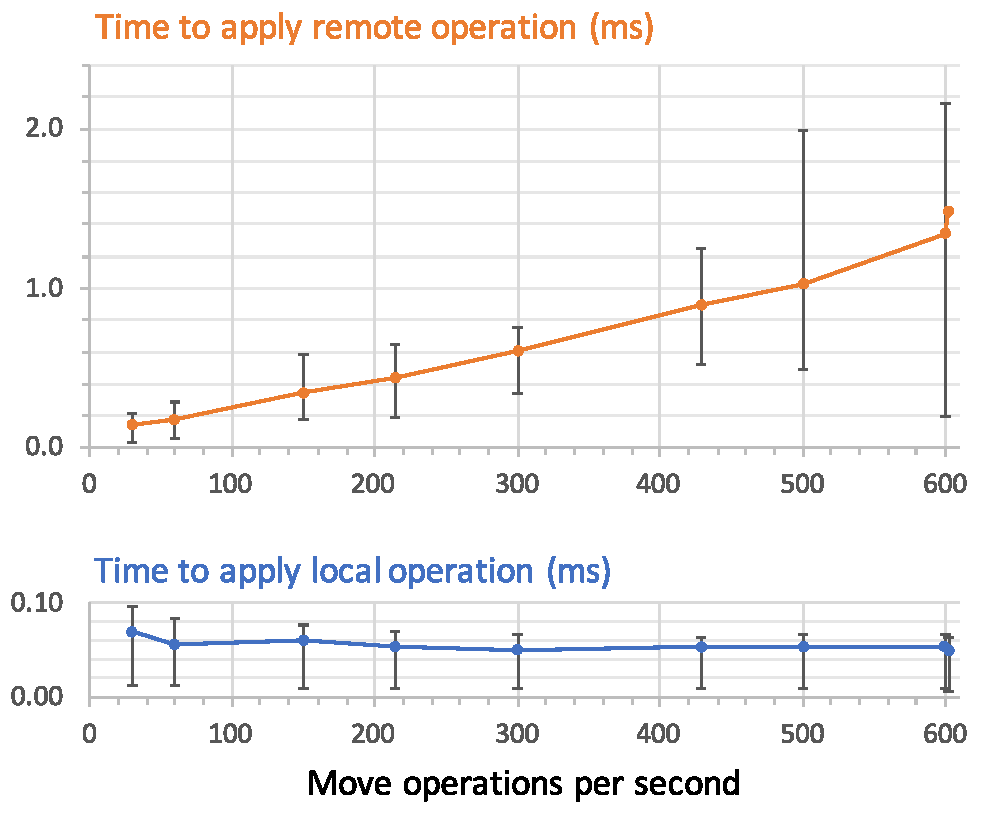
\includegraphics[width=\columnwidth,keepaspectratio=true]{plot.pdf}
  \caption{Median execution time for applying an operation to the replica state, on an Amazon EC2 c5.large instance, at varying operation throughput rates. Error bars indicate the minimum and 95th percentile execution times.}
  \label{fig:plots}
\end{figure}

\begin{figure}
  \vspace{20pt}
  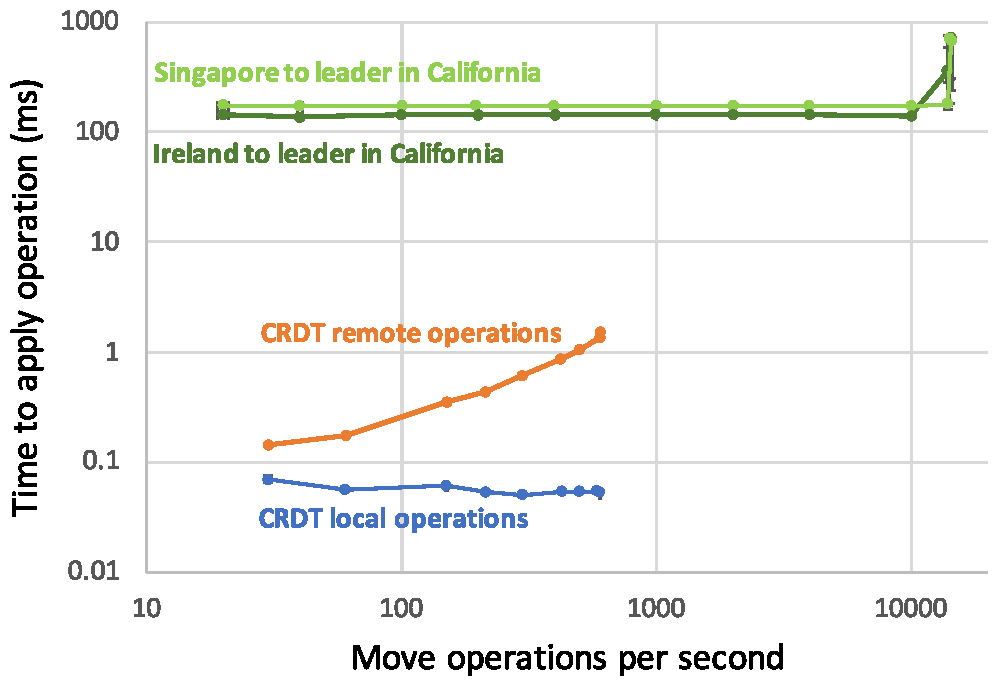
\includegraphics[width=\columnwidth,keepaspectratio=true]{leader-plot.pdf}
  \caption{Median time to apply a local CRDT operation compared to the median time to perform a move operation using state machine replication, with a leader located in another region. Note the log scale on both axes.}
  \label{fig:leader-plot}
\end{figure}

Local operations take constant time is because a locally generated operation always has a timestamp greater than any existing operation at the generating replica at that time (by definition of Lamport timestamps).
Applying that operation requires only a \isa{do\_op}, and no \isa{undo\_op} or \isa{redo\_op}.

On the other hand, for remote operations, a number of undos and redos must be performed, depending on the degree of concurrency.
As the time interval between successive operations is smaller than the network delay between replicas, there are multiple operations ``in flight'' at the same time, and more calls to \isa{undo\_op} and \isa{redo\_op} are required to order operations by timestamp.
The time taken to apply a remote operation is proportional to the number of undos and redos required, and hence proportional to the operation rate.

Note that when a user is interacting with the system, they only have to wait for local operations to execute; any remote operations can be applied in the background without affecting user interaction.
Since our algorithm need not perform any undos or redos for local operations, these user interactions are consistently fast.

\subsection{Comparison to state machine replication}\label{sec:smr}

A simple alternative to our CRDT algorithm is to use state machine replication~\cite{Schneider:1990vy}: that is, we use a leader replica or consensus algorithm to impose a total order on all operations, and then execute operations in that same order on all replicas.
For a move operation on trees, the state machine replication algorithm is much simpler than the CRDT: it still needs to check for cycles, but it never needs to undo or redo any operations because they are never applied out-of-order.

To compare the performance of our algorithm to the state machine approach we ran another set of experiments on the same three replicas in California, Ireland, and Singapore.
In this experiment, the Californian replica was designated leader; it totally ordered all operations it received, and sent them to all other replicas in the same order.
The Irish and Singaporean replicas generated operations, sent them to the leader, and applied them to their local tree in the order they were received from the leader.
In order to ensure a fair comparison to the CRDT algorithm, these experiments used the same Isabelle-generated Scala code.

The results from this experiment are shown in Figure~\ref{fig:leader-plot}.
The leader-based approach was able to sustain a throughput of 14,000 move operations per second, approximately 23 times the CRDT's throughput of 600 ops/sec (shown as an asymptote in Figure~\ref{fig:leader-plot}), due to the fact that it does not need to spend CPU cycles undoing and redoing operations.
On the other hand, the latency of each operation is much higher in the state machine approach, because the generating replica needs to wait for a round trip through the leader.
This latency is around 145~ms for operations generated in Ireland and around 176~ms for Singapore (cf. Table~\ref{tab:rpc-times}), compared with the CRDT's 50~{\textmu}s processing time for local operations.

Therefore, we have a clear trade-off: in applications that need to prioritise throughput, a state machine replication approach is preferable, while in applications that need to minimise response times to user requests, our CRDT algorithm is preferable.
Our algorithm also has the advantage that local user operations require no waiting for network communication, making them highly available in the face of network failures.
It also supports offline operation: mobile devices can read and modify their local replica of the tree even while disconnected from the Internet, which is not the case with leader-based replication.

We note that the throughput of 600 ops/sec is for a single tree, e.g.\ a filesystem belonging to one user.
Operations on independent trees, belonging to different users, can be processed in parallel.
We believe that for many applications, 600 ops/sec/user is plenty, and the ability to work offline is a valuable benefit.

\subsection{Evaluation of formal proof}

The formalisation of our algorithm, and the proofs of its properties as described in \S\ref{sec:proof}, have been formally checked by Isabelle/HOL.
Our proofs contain no unproven assumptions (i.e. no occurrences of the \textbf{sorry} keyword).
Checking all of the proofs takes 3.5 minutes on a 2018 MacBook Pro.

Besides the 60 lines of definitions given in Figure~\ref{fig:code}, our Isabelle/HOL formalisation consists of a further 2,166 lines of code.
Of this, we use 203 lines to prove that every node has a unique parent, 443 lines to prove that the tree contains no cycles, 450 lines to prove that move operations commute and replicas converge, 327 lines to prove the strong eventual consistency of our algorithm using the framework of Gomes et al.~\cite{Gomes:2017gy}, and 743 lines to define the executable variant of our algorithm (\S\ref{subsect.extracting}) and prove its equivalence to the abstract definitions of Figure~\ref{fig:code}.

\section{Related work}\label{sec:relwork}

Many replicated data systems use optimistic replication \cite{Saito:2005jw}, which allows the state of replicas to temporarily diverge, in order to achieve better performance and availability in the presence of faults than strongly consistent systems~\cite{Bailis:2014th,Gilbert:2002il}.
As a consequence, these systems require a mechanism for merging or reconciling conflicting updates that were made concurrently on different replicas.
For example, version control systems such as Git~\cite{Chacon:2014kr} leave conflicts for the user to resolve manually.
Databases such as Dynamo~\cite{DeCandia:2007ui} and Bayou~\cite{Terry:1995dn} rely on the application programmer to provide explicit conflict resolution logic; however, such logic is difficult to get right \cite{Bailis:2013jc,Burckhardt:2014hy,Gomes:2017gy}.
Hence, we focus on systems that automatically ensure that all replicas converge towards a consistent state, without requiring custom application logic---a consistency model known as \emph{strong eventual consistency}~\cite{Shapiro:2011un,Gomes:2017gy}.

\subsection{Conflict-free Replicated Data Types}

Our algorithm is an operation-based Conflict-free Replicated Data Type or CRDT~\cite{Shapiro:2011wy,Shapiro:2011un,Burckhardt:2014ft}.
All CRDTs share the property that concurrent changes on different replicas can be merged in any order; any two replicas that have seen the same set of updates are guaranteed to be in the same state, regardless of the order in which they processed these updates.
CRDTs have been defined for various abstract datatypes, such as registers and counters \cite{Shapiro:2011wy,Shapiro:2011un}, maps \cite{Baquero:2016iv,Kleppmann:2016ve}, sets \cite{Bieniusa:2012wu,Bieniusa:2012gt}, lists (sequences) \cite{Roh:2011dw,Nedelec:2013ky}, and text \cite{Preguica:2009fz,Weiss:2010hx}.
For trees, several approaches have been proposed:
\begin{itemize}
    \item Martin et al.~\cite{Martin:2010ih} define a CRDT for XML data, and Kleppmann and Beresford~\cite{Kleppmann:2016ve} define a CRDT with a JSON data model.
        However, these algorithms only deal with insertion and deletion of tree nodes, and do not support moves.
    \item As discussed in \S\ref{sec:impossibility}, Najafzadeh et al.~\cite{Najafzadeh:2017vk,Najafzadeh:2018bw} propose two implementations for a replicated filesystem: a CRDT in which conflicting moves are handled by duplicating tree nodes (as in Figures~\ref{fig:move-same-item}b and~\ref{fig:move-cycle}b), and a centralised implementation in which move operations must obtain a lock before executing (not a CRDT since it relies on synchronous coordination).
    \item Ahmed-Nacer et al.~\cite{AhmedNacer:2012us} outline approaches to handling conflicts on trees, but do not provide algorithms.
    \item Tao et al.~\cite{Tao:2015gd} propose handling conflicting move operations by allowing the same object to appear in more than one location; thus, their datatype is strictly a DAG, not a tree.
        Some conflicts are handled by duplicating tree nodes.
        Tao et al.\ also perform experiments with Dropbox, Google Drive, and OneDrive, similar to our experiments discussed in \S\ref{sec:move-is-hard}.
\end{itemize}

Besides CRDTs, another family of algorithms for concurrent modification of data structures is \emph{Operational Transformation} (OT)~\cite{Sun:1998vf}.
Several authors have defined concurrent tree structures using OT \cite{Jungnickel:2016cb,Ignat:2003jy,Davis:2002iv}, but they only consider insertion and deletion of nodes, and do not support moves.

Molli et al.~\cite{Molli:2003cd} define an OT tree structure with a move operation.
However, it requires that all communication between replicas is performed via total order broadcast, which requires a leader replica or consensus algorithm, like in \S\ref{sec:smr}.
Our algorithm has better availability characteristics in the presence of network partitions because it allows messages to be delivered in any order, e.g.\ via peer-to-peer protocols.

\subsection{Distributed filesystems}\label{sec:filesystems}

Many distributed filesystems, such as NFS, rely on synchronous interaction with a server.
This avoids the need for conflict resolution, but rules out users working offline.

Coda is a client-server filesystem that allows clients to locally cache copies of files stored in a server-side data repository~\cite{kistler1992coda}. 
Clients can edit data in the cache while offline, during which time a kernel module keeps track of all updates. 
When the client comes back online it attempts to resynchronise changes with the server. 
To resolve conflicts due to concurrent updates, Coda uses application-specific resolvers~\cite{Kumar:1995wf}, similarly to Bayou's approach~\cite{Terry:1995dn}.
Concurrent renaming and move operations have been considered, but the authors note that they do ``not address transparent resolution of cross-directory renames [i.e.\ move operations] in [their] current implementation''~\cite{kumar1993log}.
Furthermore, while the authors consider a number of conflicts associated with directory move operations, they do not highlight the potential for the creation of cycles.

Ficus~\cite{Reiher:1994wh} is an in-kernel SunOS-based replicated peer-to-peer filesystem. 
Ficus supports updates to replicas during periods of network partition and claims ``conflicting updates to directories are detected and automatically repaired''~\cite{guy1990implementation}. 
Unfortunately we were unable to find a precise definition of the algorithm used in any of the available publications. 

Rumor~\cite{Guy:1999gy,RumorManual} is the successor to Ficus.
While previous work uses the kernel filesystem interface, Rumor is a userspace process that is invoked periodically by the user or by a daemon; when run, it compares the state of the replicas.
The original version of Rumor was unable to scale beyond 20 replicas, but an extension called Roam~\cite{Ratner:1999fh} allowed better scaling. 
In an attempt to test Rumor's conflict handling we obtained the source code from \emph{archive.org}~\cite{RumorSource}; however, we were unable to get it running after modest effort.
%The user manual \cite{RumorManual} makes the claim that "Unix directories are an important example of a kind of file for which Rumor automatically resolves conflicts"

Unison is a file synchronisation tool with a formal specification that allows two replicas to synchronise the state of a directory~\cite{PierceVouillon:UnisonSpecTR}.
It permits offline updates to both replicas.
Like Rumor, Unison is a userspace process that compares replica states.
Whenever it is run, Unison records a summary of the filesystem state on each replica, and it uses this summary to determine the changes made since the last synchronisation. 
When presented with the move operations described in Figure~\ref{fig:move-same-item}, Unison duplicates the files, resulting in the outcome shown in Figure~\ref{fig:move-same-item}a. 
Unison is unable to automatically synchronise the move operations shown in Figure~\ref{fig:move-cycle} and instead asks the user to choose one of four possible resolutions: those shown in Figure~\ref{fig:move-cycle}b, \ref{fig:move-cycle}c, \ref{fig:move-cycle}d, or to delete both directories.

Hughes et al.~\cite{Hughes:2016fp} test Dropbox and Google Drive against a formal specification, but they do not consider moving files, and thus do not find the issue described in \S~\ref{sec:move-cycle}.

Bj{\o}rner~\cite{Bjorner:2007hp} discusses the development of the Distributed File System Replication (DFS-R) component of Windows Server, during which a model checker found an issue with concurrent moves similar to Figure~\ref{fig:move-cycle}a.
Bj{\o}rner outlines several possible solutions, but notes that model-checking their algorithm was not feasible due to state space explosion.
Our use of proof by induction, rather than model-checking, allows us to verify the correctness of our algorithm in unbounded executions.

\subsection{Totally ordered operation log}

Ordering operations by a timestamp, and undoing/redoing them as necessary so that they take effect in ascending timestamp order, is a well-known approach.
It is used for example in systems like Bayou~\cite{Terry:1995dn}, Jefferson's \emph{Time Warp} mechanism~\cite{Jefferson:1985em}, Shapiro et al.'s \emph{capricious total order}~\cite{Shapiro:2016hp}, and Burckhardt's \emph{standard conflict resolution}~\cite[\S~4.3.3]{Burckhardt:2014hy}.

However, to our knowledge, this approach has not previously been applied to the problem of replicated trees, nor are we aware of previous mechanised proofs (using Isabelle or other tools) that formalise this approach.

\section{Conclusions}

In this paper we have defined a novel algorithm that handles arbitrary concurrent modifications of a tree data structure -- adding, moving, and removing nodes -- in a peer-to-peer replication setting.
It is applicable to distributed filesystems and many other applications that use a tree-structured data model.
Our approach ensures that all replicas converge to the same consistent state without requiring any manual conflict resolution, and without needing application developers to implement conflict handling logic.
Updates made to a local replica take effect immediately, while operations from remote replicas can be propagated and applied in the background.
This approach means that user interaction is consistently fast, even in the face of unbounded communication delays or during disconnected operation of mobile devices.

While existing systems exhibit anomalies (such as duplicating nodes or introducing cycles) or bugs and internal errors (like in Figure~\ref{fig:gdrive-error}) in the face of concurrent move operations, our algorithm is free from such problems.
We formally verified the correctness of our algorithm using the Isabelle/HOL proof assistant; our theorems show that replicas can apply operations in any order, and that the result is always a valid tree (nodes have at most one parent, and the graph does not contain any cycles).
Moreover, these results apply to unbounded executions and an arbitrary number of replicas---an inherent advantage of using a proof assistant rather than other formal approaches such as model checking.

We also extracted a formally verified Scala implementation from our Isabelle/HOL definitions, and evaluated its performance across three replicas in California, Ireland and Singapore.
Our implementation applies local updates in approximately 50~{\textmu}s, orders of magnitude faster than is possible with a leader replica or consensus protocol operating over these distances, and it remains available in the face of network interruptions.
However, compared to leader-based replication our algorithm has lower throughput of 600 updates per second.
A hand-optimised implementation of our algorithm could achieve higher performance, since code generated from HOL definitions contains inefficiencies.
The generated code could serve as a reference implementation against which other implementations could be tested.

As mentioned in the introduction, our work is especially interesting due to the ubiquity of tree data models across many different computing systems.
In future work we hope to build novel applications, such as a distributed filesystem, using our algorithm.

\section*{Acknowledgements}

The authors wish to acknowledge the support of The Boeing Company and the EPSRC ``REMS: Rigorous Engineering for Mainstream Systems'' programme grant (EP/K008528).
Martin Kleppmann is supported by a Leverhulme Early Career Fellowship and by the Isaac Newton Trust.
Our evaluation was conducted using AWS credits from the AWS Educate program.
Thank you to Marc Shapiro for feedback on a draft of this paper.

%\balance
\bibliographystyle{abbrv}
\bibliography{references}{}
\end{document}
